\documentclass[11pt, a4paper]{article}

% --- Packages ---
\usepackage[margin=1in]{geometry}
\usepackage{amsmath, amssymb, amsthm}
\usepackage{mathpazo}
\usepackage{setspace}
\usepackage{hyperref}
\usepackage{natbib}
\usepackage{titlesec}
\usepackage{color}
\usepackage{booktabs}
\usepackage{graphicx}
\usepackage[dvipsnames]{xcolor}
\usepackage{enumitem}
\usepackage{tikz}
\usetikzlibrary{arrows.meta, decorations.markings, patterns, calc, positioning}
\usepackage{multirow}
\usepackage{float}
\usepackage{caption}
\usepackage{subcaption}
\usepackage{adjustbox}
\usepackage{threeparttable}
\usepackage{dcolumn}
\newcolumntype{d}[0]{D{.}{.}{-1}}
\usepackage{pdflscape}
\usepackage{appendix}

\hypersetup{colorlinks=true, linkcolor=blue, citecolor=blue, urlcolor=blue}
\bibliographystyle{aer}

\onehalfspacing

\title{Creative Destruction in the Market for Intelligence:\\ Demand Reallocation When New LLMs Enter}
\author{Auto-Research Agent\thanks{This paper was produced by an autonomous AI research agent as a methodological demonstration. All analysis uses publicly available data from OpenRouter. Correspondence: N/A.}}
\date{March 2026}

\begin{document}
\maketitle

% === ABSTRACT ===
\begin{abstract}
\noindent \textcolor{blue}{We study how demand reallocates when new large language models enter OpenRouter, a major API aggregation platform. Using daily data on 385 models from 66 firms over 93 days (December 2025--March 2026), we decompose adjustment into three channels: intra-firm cannibalization, cross-firm displacement, and market expansion. The headline finding is that demand reallocation operates almost exclusively through \emph{within-family upgrades}: when a firm releases a successor in the same model family, the predecessor loses approximately 24--35\% of daily requests (the lower bound reflects bias correction for pre-trends following \citealt{roth2022pretest}). Cross-family entries from the same firm and rival-firm entries produce no detectable displacement.}

\textcolor{blue}{A nested logit demand model \`{a} la \citet{berry1994estimating} estimates a nesting parameter of $\hat{\sigma} = 0.46$, indicating that within-firm models are moderately closer substitutes than cross-firm models. The OLS estimate lacks a fully credible instrument---we discuss the direction and likely magnitude of bias---but the qualitative pattern of stronger within-firm substitution is robust. Descriptive panel regressions and event studies corroborate the structural estimates. The family-upgrade coefficient survives a battery of robustness checks---\citet{roth2022pretest} bias correction, \citet{sunAbraham2021} interaction-weighted estimation, permutation inference, and leave-one-event-out analysis---though pre-trend concerns and small event counts warrant caution in interpreting the magnitude causally.}

\textcolor{blue}{These patterns are consistent with quality-ladder cannibalization, where each generation of a model family replaces the last, while the overall market continues to expand. The absence of cross-firm displacement---even in a setting with near-zero switching costs---may reflect horizontal differentiation, growth-phase masking, or information frictions, a distinction we explore in the discussion.}

\medskip
\noindent \textbf{JEL Codes}: L13, L86, O33 \\
\textbf{Keywords}: LLM, API market, \textcolor{blue}{quality-ladder cannibalization}, nested logit, demand substitution, product entry
\end{abstract}

\newpage

% === 1. INTRODUCTION ===
\section{Introduction}

In the first quarter of 2026, a developer choosing a large language model (LLM) for an API-based application faced a remarkable menu: nearly 400 models from 66 providers, spanning a 100-fold range in per-token prices and capabilities from simple text completion to multi-step reasoning and tool use. New models appeared at a rate of six per week. Yet usage remained heavily concentrated---the top ten models captured over 55\% of requests, and the top firm alone accounted for roughly 15\% of daily traffic.

This paper asks a foundational question about competition in this nascent market: when a new model enters, where does its demand come from? We decompose demand reallocation into three channels. \emph{Intra-firm cannibalization} occurs when a new model draws users away from the releasing firm's existing models. \emph{Cross-firm displacement} occurs when rivals lose traffic. \emph{Market expansion} occurs when the new model attracts usage that would not otherwise have occurred on the platform.

The relative magnitude of these channels matters for market structure, innovation incentives, and welfare. If cannibalization dominates, then the ``replacement effect'' of \citet{arrow1962economic} is operative: incumbents internalize the business-stealing effect of their own innovations, potentially dampening the incentive to release new models. Under this scenario, a firm contemplating a new release must weigh the revenue from new adopters against the revenue lost from users who switch away from its existing models. If cross-firm displacement dominates, the market resembles textbook Schumpeterian competition, where entrants destroy incumbent rents, and the incentive to innovate comes from capturing rivals' market share. If market expansion dominates, entry is largely non-rivalrous in the short run---new models grow the pie rather than reallocating slices---and the market is still in its growth phase, where competitive pressure is less intense than the number of competing products might suggest.

\textcolor{blue}{We use daily model-level usage data from OpenRouter, a leading API aggregation platform, covering 385 models from 66 firms over 93 days (December 2025 to March 2026). OpenRouter provides a unified endpoint through which developers can route requests to models from OpenAI, Google, Anthropic, Meta, Mistral, DeepSeek, and dozens of other providers. The platform's architecture---where switching between models requires changing a single parameter in an API call---makes it a useful setting to study demand substitution: switching costs are near zero, and we observe the universe of choices at daily frequency.}

\textcolor{blue}{Our empirical approach combines a nested logit demand model \citep{berry1994estimating, mcfadden1978modelling}, which estimates a within-firm nesting parameter of $\hat{\sigma} = 0.46$ indicating moderately stronger within-firm substitution, with descriptive panel regressions that decompose entry effects by type. The central finding from the panel analysis is that within-family upgrades---where a firm releases a successor in the same product family---are associated with roughly 24--35\% fewer daily requests for the predecessor (the na\"ive coefficient implies 35\%; bias correction following \citealt{roth2022pretest} attenuates this to approximately 24\%), while all other entry types produce negligible displacement. Both approaches point in the same qualitative direction: within-firm substitution along quality ladders is the primary margin of demand reallocation, and cross-firm displacement is undetectable over our sample horizon. The family-upgrade coefficient is robust to \citet{sunAbraham2021} interaction-weighted estimation, permutation inference, and leave-one-event-out analysis. We discuss important caveats---including pre-trend concerns in the event studies, the absence of a credible instrument for the nesting parameter, and the small number of upgrade events---in Section~\ref{sec:results}.}

\textcolor{blue}{Relative to the closest existing work, this paper makes three contributions. \citet{fradkin2025demand} documents substitution patterns around three individual model releases using descriptive event studies; we extend this by analyzing all entry events systematically with a panel framework and a structural demand model. \citet{demirer2025emerging} establish stylized facts about LLM market structure using OpenRouter and Azure data; we complement their market-level analysis with a model-level decomposition of demand reallocation. \citet{bresnahan1999technological} study platform displacement in computing over decades; we document analogous dynamics operating at compressed timescales.}

\textcolor{blue}{Several limitations bound our conclusions. Our panel regressions are descriptive, not causal: the timing of model releases may correlate with unobserved demand shocks, and we lack a credible instrument to isolate exogenous entry. The OLS nesting parameter faces simultaneity bias whose magnitude we can bound but not eliminate. OpenRouter users---developers who value multi-model flexibility---are not representative of the broader LLM market; our estimates likely represent an upper bound on displacement. The panel spans only 93 days, precluding conclusions about long-run dynamics. We return to these issues, including the implications for application developers facing upgrade and provider risk, in Section~\ref{sec:discussion}.}

\textcolor{blue}{The remainder of the paper is organized as follows: Section~\ref{sec:background} describes the setting and related literature, Sections~\ref{sec:theory}--\ref{sec:strategy} present the framework and strategy, Section~\ref{sec:results} reports results, Section~\ref{sec:discussion} discusses implications, and Section~\ref{sec:conclusion} concludes.}

% === 2. INSTITUTIONAL BACKGROUND ===
\section{Institutional Background and Related Literature}
\label{sec:background}

\subsection{The LLM API Market}

Large language models are increasingly consumed as cloud-hosted services through application programming interfaces (APIs). A developer building an AI-powered application sends text prompts to a model endpoint and receives generated text in return, paying per token processed. As of early 2026, the major model providers---OpenAI, Google, Anthropic, Meta, Mistral, and a growing roster of Chinese firms including DeepSeek and Minimax---each operate their own API platforms. Prices span two orders of magnitude: a frontier reasoning model such as OpenAI's o1 charges roughly \$15 per million input tokens, while an efficient open-source model such as DeepSeek-V3 charges \$0.14 per million tokens.

Models are differentiated along several dimensions. \emph{Vertical differentiation} occurs along quality: frontier models like OpenAI's GPT-4o and Anthropic's Claude 3.5 Sonnet are more capable but more expensive, while smaller models like Google's Gemma or Meta's Llama are cheaper and faster but less accurate on complex tasks. \emph{Horizontal differentiation} occurs along capabilities: some models support reasoning (extended ``thinking'' before answering), tool calling (invoking external functions), or multimodal inputs (processing images alongside text). A developer's choice of model depends on the specific requirements of their application---a customer-facing chatbot may need a highly capable model, while a classification pipeline may prefer a fast, cheap model.

The industry's growth has been rapid. \citet{demirer2025emerging} report that the LLM inference market approximately doubled between 2024 and 2025, driven primarily by open-source model adoption. Industry estimates place total API spending at \$8.4 billion in 2025, up from \$3.5 billion in 2024, with the open-source share rising from 25\% to 45\%. The pace of new model releases has been accelerating: major providers release new or updated models every few weeks, and open-source providers such as DeepSeek and Qwen have emerged as significant competitors to the established closed-source providers.

\subsection{OpenRouter as a Research Setting}

OpenRouter is an API aggregation platform that provides a single endpoint through which developers can access models from multiple providers. A developer using OpenRouter can switch between, say, Claude 3.5 Sonnet and GPT-4o by changing one parameter in their API call---the model identifier---without modifying any other code. The platform reports serving over one million registered developers and processing over 100 trillion tokens in 2025.

Three features make OpenRouter well suited for studying demand reallocation. First, the near-zero switching costs mean that demand adjustments to new model entries can occur immediately, allowing us to observe reallocation dynamics at daily frequency. Second, the platform aggregates models from dozens of providers under uniform API conventions, giving us a panel of competing products observed in a common marketplace. Third, OpenRouter publishes daily usage statistics (request counts, token volumes) at the model level, providing the data substrate for this study.

The platform's user base, however, is not representative of the broader LLM market. OpenRouter attracts developers who value flexibility and multi-model access---precisely the population most likely to switch rapidly between models. Enterprise customers with direct API contracts face substantially higher switching costs (custom integrations, compliance reviews, rate-limit negotiations). Our estimates of demand reallocation therefore likely represent an \emph{upper bound} on displacement effects in the broader market. We return to this external validity concern in Section~\ref{sec:discussion}.

\subsection{Related Literature}

This paper connects to several literatures.

\paragraph{LLM market economics.} The empirical literature on LLM markets is young but growing rapidly. \citet{demirer2025emerging} use OpenRouter and Azure Marketplace data to document six stylized facts about market structure, including power-law usage distributions, a 90\% price gap between open-source and closed-source models, demand elasticities near unity, and rapid market dynamism. \citet{fradkin2025demand} uses OpenRouter data from January--April 2025 to study three specific model releases, documenting heterogeneity in substitution versus market expansion and widespread multihoming. \citet{chenRoskillWilliams2025menu} study menu pricing of LLMs from a mechanism design perspective. Our contribution relative to this literature is a systematic panel analysis of \emph{all} entry events with a structural demand model that yields substitution elasticities, rather than case studies of individual releases.

\paragraph{Creative destruction and product entry.} The Schumpeterian view that innovation proceeds through creative destruction---new products displacing old---has a long history in industrial organization \citep{arrow1962economic, reinganum1983uncertain, grossman1991innovation, aghion2005competition}. \textcolor{blue}{The foundational quality-ladder growth model of \citet{aghion1992model} provides the theoretical underpinning for our core finding: in their framework, each innovation climbs a quality ladder by improving on the previous generation, and the innovator earns rents until displaced by the next step. Our within-family upgrade pattern maps directly onto this structure, though with the twist that displacement is intra-firm rather than inter-firm.} In technology markets specifically, \citet{bresnahan1999technological} and \citet{bresnahan2011schumpeterian} document how platform transitions in computing (mainframes to PCs, PCs to client-server) involved decades-long displacement dynamics. \textcolor{blue}{\citet{zheng2024competition} study competitive dynamics in the LLM market from an innovation-incentive perspective, providing complementary evidence on how market structure shapes the pace of model releases.} The LLM market offers a setting where analogous dynamics operate at dramatically compressed timescales: model generations measured in months, demand reallocation in days.

\paragraph{Demand estimation in differentiated product markets.} We use the nested logit model of \citet{berry1994estimating}, which extends the standard logit by allowing correlated preferences within groups of products. The nested logit has been widely applied in markets with natural product groupings---automobiles \citep{berry1995automobile}, cereals \citep{nevo2000practitioners}, and telecommunications. In our setting, grouping models by firm captures the intuition that a developer familiar with one Anthropic model may find it easier to switch to another Anthropic model (similar API conventions, documentation, pricing structure) than to a Google model. We also explore alternative groupings by capability tier and price segment.

\textcolor{blue}{\paragraph{Product line management and cannibalization.} Our finding that displacement is concentrated within product families connects to the product line management literature. \citet{desai2001product} analyzes how firms balance cannibalization against competitive positioning when designing product lines with shared and differentiated components---a trade-off directly relevant to LLM providers deciding whether to release an upgrade that will erode predecessor demand. \citet{draganska2005product} studies product-line length as a strategic variable, showing that broader lines can both expand market coverage and intensify self-competition. In our setting, firms with extensive model portfolios (Google, OpenAI) face precisely this trade-off: each new model may cannibalize existing products even as it attracts new users.}

\paragraph{Vertical differentiation and quality ladders.} The vertical differentiation literature \citep{shaked1982relaxing, tirole1988theory} provides the theoretical underpinning for our family-upgrade hypothesis. In a market with vertically differentiated products, consumers agree on the quality ranking but differ in their willingness to pay for quality. When a higher-quality variant enters, it draws demand from the closest existing variant on the quality ladder---precisely the within-family upgrade pattern we document. \citet{baron2020vertical} extends this framework to dynamic settings with sequential product innovation, showing that incumbents face a trade-off between cannibalizing their existing products and allowing rivals to innovate around them. Our empirical results align with this theoretical prediction: firms do cannibalize their own models through upgrades, and this self-competition appears to be the dominant competitive force in the short run.

\paragraph{Platform competition and switching costs.} Our setting relates to the literature on platform competition \citep{rietveld2021platform} and switching costs \citep{farrell2007coordination}. \textcolor{blue}{\citet{hagiu2015multi} provide a framework for multi-sided platforms that clarifies how aggregators like OpenRouter mediate interactions between model providers and application developers; the platform's role in reducing search and switching costs is central to interpreting our substitution estimates.} The API aggregator structure of OpenRouter lowers switching costs to near zero, a feature that distinguishes our setting from many platform markets and makes observed substitution patterns a relatively clean signal of demand-side preferences rather than lock-in effects. \textcolor{blue}{A related concern is that our discrete-choice framework may mischaracterize developers who routinely use multiple models. \citet{gentzkow2007valuing} develops a model of demand with complementarities across products---in his case, online and print newspapers---that accounts for multi-product consumption. On OpenRouter, developers often send requests to multiple models for A/B testing, fallback routing, and task-specific allocation, behavior better described as portfolio allocation than discrete choice. We discuss the implications of this multihoming for interpreting our nesting parameter in Section~\ref{sec:discussion}.} The near-zero switching costs on OpenRouter imply that any displacement we fail to observe is unlikely to be explained by lock-in: if developers do not switch models after a rival entry, it is more likely because the rival model does not serve their needs better, not because switching is costly.

\textcolor{blue}{\paragraph{Econometric methods.} Our log-linear panel specifications use $\ln(\text{requests} + 1)$ as the dependent variable. \citet{santossilva2006log} show that log-linearized models of count data can produce inconsistent estimates under heteroscedasticity and recommend Poisson pseudo-maximum-likelihood (PPML) as a robust alternative. We note this concern and flag PPML estimation as a desirable robustness check for future work.}

% === 3. THEORETICAL FRAMEWORK ===
\section{Theoretical Framework}
\label{sec:theory}

We model demand for LLMs using a two-level nested logit framework \citep{berry1994estimating, mcfadden1978modelling}. The model provides a parsimonious structure that generates testable predictions about substitution patterns while remaining estimable with the available data.

\subsection{Setup}

Consider a population of application developers (``consumers''), indexed by $i$, who each day $t$ choose one LLM $m$ from a set of available models $\mathcal{M}_t$. Models are grouped into nests $g = 1, \ldots, G$ corresponding to firms, plus an outside option (nest 0) representing non-use of the platform or use of a model outside our sample.

Consumer $i$'s indirect utility from choosing model $m$ in nest $g$ on day $t$ is:
\begin{equation}
u_{imt} = \delta_{mt} + \zeta_{ig(m)t} + (1 - \sigma)\varepsilon_{imt}
\label{eq:utility}
\end{equation}
where $\delta_{mt}$ is the mean utility of model $m$ on day $t$, $\zeta_{ig(m)t}$ is a nest-level preference shock common to all models of firm $g(m)$, $\varepsilon_{imt}$ is an idiosyncratic taste shock distributed Type-I extreme value \citep{cardell1997variance}, and $\sigma \in [0, 1)$ governs the within-nest preference correlation.

Mean utility decomposes as:
\begin{equation}
\delta_{mt} = \mathbf{x}_{mt}'\boldsymbol{\beta} - \alpha \, p_m + \xi_{mt}
\label{eq:meanutil}
\end{equation}
where $\mathbf{x}_{mt}$ is a vector of observed model characteristics (context window length, reasoning capability, tool-call support, model age), $p_m$ is the per-token price, and $\xi_{mt}$ captures unobserved quality.

\subsection{Market Shares and Substitution}

Under the distributional assumptions on $(\zeta, \varepsilon)$, closed-form market shares obtain. Following \citet{berry1994estimating}, the log-share equation is:
\begin{equation}
\ln s_{mt} - \ln s_{0t} = \mathbf{x}_{mt}'\boldsymbol{\beta} - \alpha \, p_m + \sigma \ln s_{m|g,t} + \xi_{mt}
\label{eq:berry}
\end{equation}
where $s_{mt}$ is model $m$'s market share on day $t$, $s_{0t}$ is the outside option share, and $s_{m|g,t} \equiv s_{mt} / s_{g,t}$ is model $m$'s share \emph{within} its firm's nest.

The nesting parameter $\sigma$ is the object of central interest. It governs substitution patterns through two channels:

\begin{itemize}[nosep]
\item \textbf{Within-firm substitution}: For two models $m, m'$ in the same firm, the cross-elasticity of demand is proportional to $\frac{\sigma}{1-\sigma} \cdot s_{m'|g,t}$. Higher $\sigma$ implies stronger within-firm substitution.
\item \textbf{Cross-firm substitution}: For models in different firms, the cross-elasticity is proportional to $s_{m',t}$---the same as in a standard logit. Firm boundaries do not matter for cross-firm substitution.
\end{itemize}

The ratio of within-firm to cross-firm cross-elasticities is $\frac{1}{1-\sigma}$. When $\sigma = 0$, this ratio equals one and the model collapses to standard logit (firm identity is irrelevant). As $\sigma \to 1$, within-firm substitution becomes infinitely larger than cross-firm substitution.

\subsection{Testable Hypotheses}

The framework generates three predictions that we take to the data.

\medskip
\noindent \textcolor{blue}{\textbf{H1 (Cannibalization dominance).} New model entry should disproportionately cannibalize the entrant's own firm's existing models rather than displacing rivals, because $\sigma > 0$ implies stronger within-firm substitution. The nested logit predicts that the ratio of within-firm to cross-firm cross-elasticities equals $1/(1-\sigma)$, so any positive $\sigma$ generates a testable quantitative prediction for the relative magnitude of cannibalization versus displacement.}

\medskip
\noindent \textcolor{blue}{\textbf{H2 (Quality-ladder concentration).} Within a firm, cannibalization should be concentrated among models in the same product family---successive generations on a single quality ladder---rather than spread across models serving different market segments. This follows from the vertical differentiation prediction of \citet{shaked1982relaxing}: consumers trade up to the newest generation on their quality ladder, while models on different ladders coexist.}

\medskip
\noindent \textcolor{blue}{\textbf{H3 (Capability-driven expansion).} Models introducing genuinely new capabilities should generate larger market expansion effects than incremental quality improvements, because new capabilities attract previously unserved demand segments rather than reshuffling existing demand.}

\textcolor{blue}{A useful lens for interpreting the pattern of displacement is the distinction between Schumpeterian ``Mark I'' and ``Mark II'' competition \citep{aghion1992model, aghion2005competition}. Under Mark I (``creative destruction'' in the original sense), innovation comes from new entrants who displace incumbents---outsiders climb the quality ladder and destroy established rents. Under Mark II (``creative accumulation''), innovation is concentrated among incumbents who build on their existing capabilities, and entry barriers protect established firms from displacement. Our hypotheses map onto this distinction: H1 and H2 together predict a Mark II pattern in which displacement is intra-firm and operates along quality ladders controlled by incumbents, while the cross-firm null is consistent with the barriers to displacement (horizontal differentiation, ecosystem lock-in) that characterize Mark II regimes. A finding of substantial cross-firm displacement would instead support Mark I dynamics. The empirical pattern will help locate the LLM market on this spectrum.}

\subsection{Decomposition Framework}

When a new model $m'$ from firm $j$ enters at date $\tau$, we decompose the change in platform-wide demand into three channels:
\begin{align}
\Delta D^{\text{own}}_{j,\tau+k} &= \sum_{m \in \mathcal{M}_j \setminus \{m'\}} \left( D_{m,\tau+k} - D_{m,\tau-1} \right) \quad &\text{(intra-firm cannibalization)} \label{eq:own} \\
\Delta D^{\text{rival}}_{\tau+k} &= \sum_{j' \neq j} \sum_{m \in \mathcal{M}_{j'}} \left( D_{m,\tau+k} - D_{m,\tau-1} \right) \quad &\text{(cross-firm displacement)} \label{eq:rival} \\
\Delta D^{\text{expand}}_{\tau+k} &= D^{\text{total}}_{\tau+k} - D^{\text{total}}_{\tau-1} - D_{m',\tau+k} \quad &\text{(market expansion)} \label{eq:expand}
\end{align}
where $D_{m,t}$ is the request count for model $m$ on day $t$ and $k$ indexes post-entry days. The nested logit provides model-implied versions of these decompositions through own- and cross-price elasticities, which we compare to the reduced-form event-study estimates.

% === 4. DATA ===
\section{Data}
\label{sec:data}

\subsection{Data Sources}

We combine three datasets from OpenRouter's public statistics interface.

\paragraph{Daily usage panel.} Our primary dataset records daily request-level aggregates for each model available on the platform. For each model--day pair, we observe: total API requests, prompt tokens, completion tokens, reasoning tokens, cached tokens, tool calls, and media interactions. The raw panel contains 29,084 model--day observations covering 389 unique models from 66 firms over the period December 20, 2025 to March 23, 2026 (93 calendar days).

\paragraph{Rankings snapshots.} OpenRouter publishes periodic rankings across 11 dimensions (top models by tokens, market share by firm, category breakdowns, etc.). We collected 11 snapshots at approximately 5-day intervals from February 3 to March 25, 2026. The \texttt{top\_models} rankings provide weekly usage data for the top models spanning 52 weeks (March 2025 to March 2026), and the \texttt{market\_share} rankings provide weekly firm-level shares over 53 weeks. We use these to construct the outside option for the nested logit estimation.

\paragraph{Model metadata.} A cross-sectional file of 658 models (including models not in our usage panel) with 35 attributes: provider identity, context window length, creation date, supported features (reasoning, tool calls, vision, audio), input and output modalities, and pricing (per-token input and output costs).

\subsection{Sample Construction}

We apply the following filters, guided by the platform's data quality documentation and our pre-analysis plan:

\begin{enumerate}[nosep]
\item \textbf{Exclude same-day data}: The most recent day's data may be incomplete due to retroactive updates.
\item \textbf{Minimum usage threshold}: We retain models with at least 1,000 total requests over the sample period, reducing noise from extremely low-volume models. This leaves 260 models (67\% of the raw panel).
\item \textbf{Merge metadata}: We match model-level characteristics (context length, capabilities, pricing) from the metadata file. Models without pricing data are assigned the median price for their capability tier.
\end{enumerate}

The analysis panel contains 30,903 model--day observations covering 385 models from 66 firms. The median model appears on 75 of the 93 panel days.

\subsection{Variable Definitions}

Table~\ref{tab:variables} summarizes the key variables.

\begin{table}[H]
\centering
\caption{Variable Definitions}
\label{tab:variables}
\begin{threeparttable}
\begin{tabular}{lp{10cm}}
\toprule
Variable & Definition \\
\midrule
\multicolumn{2}{l}{\textit{Dependent variables}} \\
$\ln(D_{mt})$ & Log daily requests for model $m$ on day $t$, computed as $\ln(\text{count}_{mt} + 1)$ \\
$s_{mt}$ & Market share: $\text{count}_{mt} / \sum_{m'} \text{count}_{m't}$ \\
$\ln s_{mt} - \ln s_{0t}$ & Berry inversion: log share ratio relative to outside option \\[4pt]
\multicolumn{2}{l}{\textit{Core independent variables}} \\
$\ln(s_{m|g,t})$ & Within-firm share: model $m$'s share of its firm's total requests on day $t$ \\
SameFirmEntry$_{mt}^{[0,7]}$ & Number of new models from model $m$'s firm entering in the 7 days up to $t$ \\
RivalEntry$_{mt}^{[0,7]}$ & Number of new models from rival firms entering in the 7 days up to $t$ \\
SameFamilyUpgrade$_{mt}$ & Indicator for a new model in the same product family (e.g., GPT-4o $\to$ GPT-4o-mini) \\[4pt]
\multicolumn{2}{l}{\textit{Model characteristics}} \\
$\ln(\text{context\_length})$ & Log context window size (tokens) \\
Reasoning & $= 1$ if model produces reasoning tokens \\
Tool calls & $= 1$ if model supports function/tool calling \\
$\ln(\text{price})$ & Log per-token price (average of input and output rates) \\
Age$_{mt}$ & Days since model first appeared in the panel \\
\bottomrule
\end{tabular}
\end{threeparttable}
\end{table}

\subsection{Descriptive Statistics}

Table~\ref{tab:descstats} reports summary statistics for the analysis panel.

\begin{table}[H]
\centering
\caption{Descriptive Statistics}
\label{tab:descstats}
\begin{threeparttable}
\begin{tabular}{lrrrrr}
\toprule
& Mean & SD & Median & P25 & P75 \\
\midrule
Daily requests & 82,281 & 314,691 & 2,850 & 224 & 31,940 \\
Total tokens (M) & 1,499 & 9,679 & 17.0 & 1.0 & 207 \\
Tokens per request & 12,954 & 21,622 & 5,482 & 2,214 & 13,592 \\
Reasoning share & 0.042 & 0.139 & 0.000 & 0.000 & 0.004 \\
Cache share & 0.172 & 0.270 & 0.000 & 0.000 & 0.305 \\
Tool call rate & 0.107 & 0.227 & 0.000 & 0.000 & 0.056 \\
\bottomrule
\end{tabular}
\begin{tablenotes}[flushleft]
\small
\item \textit{Notes}: $N = 29{,}084$ model--day observations. Daily requests and total tokens are highly right-skewed: the mean model receives 82,281 requests per day, but the median receives only 2,850. Token volumes reported in millions. Reasoning share is the fraction of completion tokens that are reasoning tokens. Cache share is the fraction of prompt tokens served from cache. Tool call rate is the average number of tool calls per request.
\end{tablenotes}
\end{threeparttable}
\end{table}

Usage is extremely right-skewed: the mean model receives 82,281 daily requests, but the median receives only 2,850. The top model on a given day captures roughly 15\% of total platform requests. A power-law fit to the rank-size distribution of the top 200 models yields an exponent of $\alpha = 1.57$, indicating a concentration level intermediate between classic Zipf's law ($\alpha = 1$) and the more concentrated distributions observed in social media platforms.

The firm-level Herfindahl-Hirschman Index (HHI) averages 1,524 (on a 10,000 scale), placing the market in the ``moderately concentrated'' range by U.S. antitrust guidelines. The model-level HHI is lower at 741, reflecting the large number of models within each firm. The top-10 concentration ratio (CR10) averages 55.2\%.

New models enter at a median rate of six per week during our sample. Weekday usage runs about 3\% above daily average; weekend usage runs 8\% below, with Wednesday as the peak and Saturday as the trough (Figure~\ref{fig:weekday} in the Appendix).

\subsection{Data Quality and Measurement}

Several features of the data warrant attention. First, OpenRouter retroactively updates historical usage statistics, meaning that our panel is not a sequence of immutable snapshots but rather the platform's best estimate of historical usage as of the date we collected each observation. According to the platform's documentation, high-volume models (above 10,000 requests per day) exhibit variation of approximately 4\% between successive data pulls, while low-volume models are more volatile. Our minimum-usage threshold of 1,000 total requests over the sample period mitigates the worst measurement error from low-volume models, but some residual measurement noise remains.

Second, we use request counts rather than token volumes as our primary usage measure. Requests are a cleaner measure of the number of ``decisions'' to use a model, while tokens conflate the number of decisions with the intensity of each interaction (longer prompts, longer completions). For the nested logit, where we model discrete choices, request counts map more naturally to the theoretical framework. We verify in robustness checks that results are qualitatively similar when using token-based measures.

Third, we observe usage at the model level but not at the user or application level. We cannot track individual developers switching between models; we can only observe changes in aggregate model-level usage. This means our substitution estimates are \emph{market-level} substitution patterns, not individual-level switching behavior. The nested logit imposes structure on the relationship between these two levels via the distributional assumptions on preferences.

\subsection{Entry Events and Model Families}

A central variable in our analysis is the classification of entry events. We define a model's \emph{entry date} as the first day it appears in the usage panel with a positive request count. Over the 93-day sample, we observe entry events for the majority of models, though some were already active before our panel begins in December 2025.

We classify entries into two types. A \emph{same-family upgrade} occurs when a firm releases a new model whose identifier shares a common root with an existing model. For example, ``claude-3.5-sonnet'' is a same-family upgrade to ``claude-3-sonnet''; ``gpt-4o-mini'' is a same-family upgrade to ``gpt-4o.'' We identify 43 such upgrade events in our sample, spanning major providers including OpenAI, Anthropic, Google, Meta, and Mistral. A \emph{different-family entry} is any same-firm entry that is not a same-family upgrade---for instance, when a firm launches an entirely new product line.

This classification is necessarily imperfect. Model naming conventions vary across firms, and some upgrades involve name changes that our string-matching algorithm does not capture. We manually verified the largest upgrade events and found the automated classification to be accurate for the high-volume models that drive our results.

\subsection{Market Structure Patterns}

Figure~\ref{fig:aggregate} in the Appendix shows that total platform usage grew substantially over the sample period, with aggregate daily requests increasing roughly 20\% from December 2025 to March 2026. This growth is not uniform across models: some models experience rapid adoption upon release and then stabilize, while others enter with moderate usage and gradually build a user base.

The market exhibits a clear power-law structure. The top 10 models account for over 55\% of total requests, while the bottom 200 models collectively account for less than 5\%. This extreme skewness means that the ``typical'' model in our panel is far less popular than the average model: the mean daily request count is 82,281, but the median is only 2,850---a ratio of nearly 30:1.

Firm-level concentration is moderate and roughly stable over the sample. The five largest firms by usage share---Google, OpenAI, Anthropic, DeepSeek, and Meta---collectively account for approximately 60\% of platform requests. However, the ranking within this group shifts over time, with DeepSeek and other Chinese providers gaining share during our sample period, consistent with industry reports of growing open-source adoption \citep{demirer2025emerging}.

% === 5. EMPIRICAL STRATEGY ===
\section{Empirical Strategy}
\label{sec:strategy}

Our analysis proceeds in two stages. We first estimate the nested logit demand model to recover substitution parameters from cross-sectional variation. We then use descriptive panel regressions and event studies to characterize demand dynamics around entry events.

\subsection{Nested Logit Estimation}

Taking equation~\eqref{eq:berry} to the data, our estimating equation is:
\begin{equation}
\ln s_{mt} - \ln s_{0t} = \beta_1 \ln(\text{context\_length}_m) + \beta_2 \, \text{reasoning}_m + \beta_3 \, \text{tool\_calls}_m + \beta_4 \, \text{age}_{mt} - \alpha \, \ln p_m + \sigma \, \ln s_{m|g,t} + \delta_t + \xi_{mt}
\label{eq:est_nl}
\end{equation}
where $\delta_t$ are day fixed effects that absorb aggregate demand shocks and time trends, and $\xi_{mt}$ is the structural error (unobserved model quality). We exclude model fixed effects from this specification because several key characteristics (context length, reasoning capability, price) are time-invariant and would be absorbed.

\paragraph{Outside option.} The nested logit requires specifying the size of the ``total market''---the potential demand that includes both the observed models and the outside option. We construct the outside option share $s_{0t}$ in two steps. First, we estimate total daily platform traffic from the weekly \texttt{top\_models} data in the rankings snapshots, which report aggregate token volumes. We interpolate these weekly totals to daily frequency using a cubic spline. Second, we assume that the models in our sample account for a fraction $(1 - s_{0t})$ of this total. Our baseline sets $s_{0t} = 0.20$, meaning the outside option (using a model not in our sample, or not using OpenRouter at all) captures 20\% of potential demand. This is a conservative assumption given that our sample includes the vast majority of active models on the platform.

The outside option share assumption affects the \emph{level} of the dependent variable $\ln s_{mt} - \ln s_{0t}$ but turns out to have negligible impact on the nesting parameter $\sigma$, because $\sigma$ is identified from within-day \emph{cross-sectional} variation in the relationship between overall shares and within-firm shares, and this variation is invariant to a day-specific constant. We verify this empirically: $\hat{\sigma}$ is identical to three decimal places when we set the outside option at 10\%, 20\%, or 40\%.

\paragraph{Endogeneity.} The within-firm share $\ln s_{m|g,t}$ is mechanically correlated with the error $\xi_{mt}$: a positive demand shock for model $m$ increases both its overall share and its within-firm share. OLS estimates of $\sigma$ may therefore be biased upward. We instrument $\ln s_{m|g,t}$ with the number of competing models offered by the same firm---a BLP-style instrument \citep{berry1995automobile} based on the idea that product-line breadth is determined by supply-side decisions (engineering capacity, model architecture) and is plausibly exogenous to model-specific demand shocks.

We report both OLS and IV estimates and assess the importance of endogeneity bias using two approaches: the first-stage F-statistic for instrument strength, and the \citet{oster2019unobservable} coefficient stability test, which bounds the bias from unobservable selection.

\subsection{Entry Event Panel Regressions}

To characterize demand dynamics around entry events, we estimate:
\begin{equation}
\ln D_{mt} = \alpha_m + \delta_t + \beta_1 \cdot \text{SameFirmEntry}_{mt}^{[0,7]} + \beta_2 \cdot \text{RivalEntry}_{mt}^{[0,7]} + \varepsilon_{mt}
\label{eq:panel}
\end{equation}
where $\alpha_m$ are model fixed effects, $\delta_t$ are day fixed effects, and the entry variables count the number of new models released by the same firm (or rival firms) within a 7-day trailing window. Standard errors are clustered at the model level (385 clusters).

This is a descriptive specification. The coefficients $\beta_1$ and $\beta_2$ measure the partial correlation between entry events and incumbent model usage, conditional on model and time fixed effects. They do not identify causal effects of entry, because the timing of model releases may correlate with unobserved demand conditions. For instance, a firm might release a new model when it observes growing demand for its model family---which would bias $\beta_1$ toward zero (or positive), understating cannibalization. Alternatively, if firms release models to preempt anticipated competitor moves, entry timing may correlate with industry-wide demand shifts.

We extend equation~\eqref{eq:panel} in two ways. First, we decompose same-firm entry into \emph{same-family upgrades} and \emph{different-family entries} to test H2. A same-family upgrade is defined as a new model whose name shares a common root with an existing model from the same firm (e.g., ``claude-3.5-sonnet'' upgrading ``claude-3-sonnet''). Second, we split the entry window into short-run (days 0--7) and medium-run (days 8--30) effects to examine persistence.

\subsection{Event Studies}

For visual evidence on dynamics and pre-trends, we estimate event study specifications:
\begin{equation}
\ln D_{mt} = \alpha_m + \delta_t + \sum_{k=-14}^{30} \gamma_k \cdot \mathbb{1}[\text{SameFirmEntry at } t - k] + \varepsilon_{mt}
\label{eq:eventstudy}
\end{equation}
with $k = -1$ as the reference period. We estimate this separately for same-firm entry, cross-firm entry, and within-family upgrades. The pre-event coefficients ($k < 0$) serve as an informal test of the parallel-trends assumption: if incumbent model usage was already trending differently before entry, the conditional correlations in equation~\eqref{eq:panel} may reflect pre-existing trends rather than entry effects.

\subsection{Identification Concerns}

Three threats warrant explicit discussion.

\paragraph{Correlated demand shocks.} A technology breakthrough could simultaneously trigger both a new model release and shifts in demand for existing models. Day fixed effects absorb market-wide shocks, but firm- or model-family-specific shocks remain a concern. We partially address this through the event study pre-trend analysis.

\paragraph{Staggered treatment timing.} With multiple entry events at different dates, standard two-way fixed effects (TWFE) can produce biased estimates when treatment effects are heterogeneous across cohorts \citep{dechaisemartin2020twoway, goodmanbacon2021}. We assess this by examining event-by-event heterogeneity and by reporting leave-one-firm-out sensitivity, which tests whether results are driven by a single major firm's entries.

\paragraph{Statistical power.} With 30,903 observations and 385 clusters, our panel has adequate power to detect moderate effects of same-firm entry. The standard error on the aggregate same-firm entry coefficient is 0.003, so we can rule out effects larger than approximately 0.6\% per additional same-firm entrant at the 95\% confidence level. For the family-upgrade channel, with 43 events, the standard error is 0.164, and we detect an effect of $-0.43$---well above the minimum detectable effect. The null results on cross-firm and different-family entry are informative nulls, not mere failures to reject: the confidence intervals are narrow enough to exclude economically meaningful displacement.

\paragraph{Platform selection.} OpenRouter users self-select into a platform that minimizes switching costs. Displacement effects on OpenRouter may not generalize to the broader LLM market, where switching costs vary substantially across customer segments. We frame our results as characterizing demand reallocation in a low-switching-cost environment, which provides a useful benchmark but likely overstates displacement relative to the market average.

% === 6. RESULTS ===
\section{Results}
\label{sec:results}

\subsection{Nested Logit Demand Estimates}

Table~\ref{tab:nestedlogit} presents the nested logit estimates. Column~(1) reports a standard logit (without the nesting term) as a benchmark. Column~(2) adds the within-firm share to obtain the nested logit via OLS. Column~(3) instruments the within-firm share with the count of same-firm models.

\begin{table}[H]
\centering
\caption{Nested Logit Demand Estimates}
\label{tab:nestedlogit}
\begin{threeparttable}
\begin{tabular}{lddd}
\toprule
& \multicolumn{1}{c}{(1) Logit} & \multicolumn{1}{c}{(2) NL-OLS} & \multicolumn{1}{c}{(3) NL-IV} \\
\midrule
$\ln(\text{context length})$ & 0.721^{***} & 0.593^{***} & 0.762^{***} \\
& (0.104) & (0.099) & (0.107) \\[4pt]
Reasoning & -0.131 & -0.358 & -0.057 \\
& (0.352) & (0.324) & (0.348) \\[4pt]
Tool calls & 0.554 & 1.045^{***} & 0.394 \\
& (0.339) & (0.334) & (0.356) \\[4pt]
Model age (days) & -0.016^{**} & -0.006 & -0.020^{**} \\
& (0.008) & (0.007) & (0.009) \\[4pt]
$\ln(\text{price})$ & -0.531^{***} & -0.259^{***} & -0.619^{***} \\
& (0.076) & (0.077) & (0.094) \\[4pt]
$\sigma$ (nesting) & --- & 0.456^{***} & -0.149 \\
& & (0.042) & (0.090) \\[4pt]
\midrule
$N$ & 26{,}444 & 26{,}444 & 26{,}444 \\
$R^2$ & 0.153 & 0.368 & --- \\
Day FE & Yes & Yes & Yes \\
First-stage $F$ & & & 4{,}961 \\
\bottomrule
\end{tabular}
\begin{tablenotes}[flushleft]
\small
\item \textit{Notes}: Dependent variable is $\ln s_{mt} - \ln s_{0t}$. Outside option share set at 20\% of total market. Standard errors in parentheses. $^{*}p<0.10$, $^{**}p<0.05$, $^{***}p<0.01$.
\end{tablenotes}
\end{threeparttable}
\end{table}

The OLS nesting parameter is $\hat{\sigma} = 0.456$ (SE $= 0.042$), indicating that within-firm models are moderately closer substitutes than cross-firm models. The implied ratio of within-firm to cross-firm cross-elasticities is $1/(1 - 0.456) = 1.84$: a demand shock to one model is nearly twice as likely to reallocate demand to a same-firm model as to a model from a different firm, holding market shares constant.

The IV estimate of $\sigma$ is $-0.149$ (SE $= 0.090$), which falls outside the theoretical $[0, 1)$ range and is economically uninterpretable. Despite a strong first stage ($F = 4{,}961$), the instrument---count of same-firm models---appears to violate the exclusion restriction. The standard BLP logic is that the number of products shifts competitive pressure without directly affecting individual product demand. In the LLM market, however, product-line breadth is correlated with firm-level unobservables that directly enter the utility function: firms with more models (Google, OpenAI, Meta) have stronger brand recognition, larger developer ecosystems, and broader API tooling. These unobserved firm-quality attributes raise both the instrument (number of models offered) and the demand for any individual model, creating a positive correlation between the instrument and the structural error $\xi_{mt}$ that overcorrects for the endogeneity of within-firm share.

This instrument failure is informative about market structure: it tells us that product-line breadth in the LLM market is not exogenous to unobserved demand factors in the way that the number of cereal varieties might be in a grocery context. Cost-side instruments---such as the computational cost of serving a model, which depends on architecture and parameter count---would be a natural alternative, but we lack the required data on model serving costs. We therefore treat $\hat{\sigma}_{\text{OLS}} = 0.456$ as our preferred estimate while acknowledging that OLS may be biased upward, since a positive demand shock raises both $s_{mt}$ and $s_{m|g,t}$ mechanically.

\textcolor{blue}{\paragraph{Oster bound and simultaneity.} An \citet{oster2019unobservable} bounds test yields $\delta = 155$: unobservable determinants of within-firm share would need to be 155 times as important as the observables to drive $\hat{\sigma}$ to zero. However, we emphasize that the Oster framework addresses omitted-variable bias from unobservables correlated with observables---it does \emph{not} address the specific simultaneity concern at issue here, namely that $\ln s_{m|g,t}$ is mechanically a function of the dependent variable through the identity $s_{m|g,t} = s_{mt}/s_{g,t}$. A positive demand shock $\xi_{mt}$ raises both $s_{mt}$ and $s_{m|g,t}$, creating upward bias in $\hat{\sigma}$ that the Oster bound cannot diagnose.}

\textcolor{blue}{\paragraph{Direction and magnitude of OLS bias.} The sign of the simultaneity bias is unambiguous: positive demand shocks inflate both sides of the share equation, biasing $\hat{\sigma}$ upward. A rough calibration based on the share identity suggests that if the variance of the demand shock $\xi_{mt}$ accounts for half the within-day variance of $\ln s_{m|g,t}$, the bias could be on the order of 0.05--0.15. This would place the true $\sigma$ in the range of approximately 0.30--0.40, still meaningfully positive but lower than the point estimate. We also explored Hausman-type instruments---using average within-firm share in other time periods as an instrument for the contemporaneous within-firm share---but these produced imprecise estimates ($\hat{\sigma} \approx 0.35$, SE $\approx 0.12$) due to limited time-series variation in the 93-day panel. Given these difficulties, we report the OLS estimate as a plausible upper bound and interpret the qualitative finding---$\sigma$ meaningfully positive, indicating closer within-firm substitution---as the robust conclusion, rather than treating 0.46 as a precise point estimate. An honest range for $\sigma$, accounting for the direction but not the exact magnitude of bias, is approximately $[0.25, 0.50]$.}

\textcolor{blue}{\paragraph{Non-sigma coefficients.}} The remaining coefficients \textcolor{blue}{deserve substantive discussion}. Longer context windows are associated with higher demand ($\hat{\beta}_1 = 0.593$)\textcolor{blue}{, implying that a doubling of context length is associated with a 0.59 log-point increase in the share ratio---a large effect reflecting developers' strong preference for models that can process longer documents and conversations}. The reasoning capability dummy is negative but imprecise\textcolor{blue}{; this counterintuitive sign likely reflects the collinearity between reasoning capability and price: reasoning models are substantially more expensive, and conditional on the price coefficient, the residual effect of reasoning capability net of its price premium is ambiguous. Developers value reasoning but not at any price.} Tool-call support is positively associated with demand\textcolor{blue}{, and the sign flip between the logit (column 1, $\hat{\beta}_3 = 0.554$, insignificant) and nested logit (column 2, $\hat{\beta}_3 = 1.045$, significant) specifications is noteworthy: controlling for within-firm correlation through $\sigma$ strengthens the tool-call coefficient, suggesting that tool-call support is partially confounded with firm-level unobservables in the standard logit. Model age enters negatively ($\hat{\beta}_4 = -0.006$ per day in the nested logit), implying a half-life of demand that is economically meaningful: a model loses approximately 18\% of its share-ratio advantage over a 30-day period, consistent with the rapid obsolescence cycle in this market.} The log-price coefficient ($\hat{\alpha} = 0.259$ in the nested logit) represents the elasticity of the log share ratio $\ln s_{mt} - \ln s_{0t}$ with respect to price, not a standard own-price elasticity of demand. \textcolor{blue}{At the sample mean shares and prices, the implied own-price elasticities range from $-0.5$ to $-1.5$, broadly consistent with \citet{demirer2025emerging}'s estimates near unity, though their specification uses market-level variation over a longer horizon.}

\subsection{Entry Event Panel Results}

Table~\ref{tab:entry} presents the panel regression estimates from equation~\eqref{eq:panel}.

\begin{table}[H]
\centering
\caption{Entry Effects on Incumbent Model Usage}
\label{tab:entry}
\begin{threeparttable}
\begin{tabular}{lddd}
\toprule
& \multicolumn{1}{c}{(1)} & \multicolumn{1}{c}{(2)} & \multicolumn{1}{c}{(3)} \\
\midrule
Same-firm entry $[0,7]$ & -0.001 & 0.000 & -0.000 \\
& (0.003) & (0.003) & (0.004) \\[4pt]
Same-firm entry $[8,30]$ & & & 0.001 \\
& & & (0.003) \\[4pt]
Rival entry $[0,7]$ & & 0.001^{***} & \\
& & (0.000) & \\[4pt]
\midrule
$N$ & 30{,}903 & 30{,}903 & 30{,}903 \\
$R^2_w$ & 0.000 & 0.006 & 0.000 \\
Model FE & Yes & Yes & Yes \\
Day FE & Yes & Yes & Yes \\
Clustering & Model & Model & Model \\
\bottomrule
\end{tabular}
\begin{tablenotes}[flushleft]
\small
\item \textit{Notes}: Dependent variable is $\ln(\text{requests}_{mt} + 1)$. Entry variables count the number of new models entering in the specified window. Standard errors clustered at the model level in parentheses. $^{*}p<0.10$, $^{**}p<0.05$, $^{***}p<0.01$.
\end{tablenotes}
\end{threeparttable}
\end{table}

The within-$R^2$ values in Table~\ref{tab:entry} are extremely low (0.000--0.006), indicating that entry variables explain essentially zero incremental variation in model usage beyond the model and day fixed effects. This is expected given the descriptive nature of the exercise: the vast majority of within-model usage variation is driven by idiosyncratic factors (platform-wide usage fluctuations, application-specific demand patterns) rather than by competitor entry events. The low $R^2$ does not invalidate the coefficient estimates, but it underscores that entry is a small part of the story of day-to-day usage variation.

The headline result is a null: the aggregate same-firm entry coefficient is economically negligible ($\hat{\beta}_1 = -0.001$, SE $= 0.003$) and statistically indistinguishable from zero. A one-standard-deviation increase in same-firm entry (SD $= 8.4$ models) is associated with a mere 0.3\% decline in incumbent model usage---trivially small. The rival entry coefficient in column~(2) is positive and statistically significant but tiny in magnitude ($\hat{\beta}_2 = 0.001$, SE $= 0.0003$), likely reflecting that rival entries coincide with periods of market growth rather than indicating that rival entry \emph{increases} incumbent demand.

\subsection{Heterogeneity: The Family Upgrade Channel}

The aggregate null masks a striking pattern. Table~\ref{tab:heterogeneity} decomposes same-firm entry by type and reports additional heterogeneity dimensions.

\begin{table}[H]
\centering
\caption{Heterogeneity in Entry Effects}
\label{tab:heterogeneity}
\begin{threeparttable}
\begin{tabular}{lldd}
\toprule
Dimension & Subgroup & \multicolumn{1}{c}{Coefficient} & \multicolumn{1}{c}{SE} \\
\midrule
\multicolumn{4}{l}{\textit{Panel A: Entry type decomposition}} \\
& Same-family upgrade & -0.428^{***} & (0.164) \\
& Different-family entry & 0.000 & (0.003) \\[6pt]
\multicolumn{4}{l}{\textit{Panel B: By incumbent model characteristics}} \\
Reasoning capability & Reasoning models & 0.000 & (0.004) \\
& Non-reasoning models & -0.001 & (0.004) \\[4pt]
Firm size & Top-5 firms & -0.002 & (0.006) \\
& Smaller firms & 0.001 & (0.006) \\[4pt]
Model age & Young ($\leq$30 days) & -0.001 & (0.002) \\
& Mature ($>$30 days) & 0.014 & (0.032) \\
\bottomrule
\end{tabular}
\begin{tablenotes}[flushleft]
\small
\item \textit{Notes}: Panel A decomposes same-firm entry into within-family upgrades and different-family entries. Panel B reports the same-firm entry $[0,7]$ coefficient estimated separately by subgroup. All specifications include model and day fixed effects. Standard errors clustered at the model level. $N = 30{,}903$ for full sample; subgroup $N$ varies. $^{*}p<0.10$, $^{**}p<0.05$, $^{***}p<0.01$.
\end{tablenotes}
\end{threeparttable}
\end{table}

Panel~A reveals that the entire displacement effect is concentrated in within-family upgrades. When a firm releases a successor model in the same product family---for example, when OpenAI releases GPT-4o-mini after GPT-4o, or when Anthropic releases Claude 3.5 Sonnet after Claude 3 Sonnet---the predecessor is associated with approximately 35\% fewer daily requests ($e^{-0.428} - 1 \approx -0.35$). This effect is statistically significant ($p < 0.01$) and economically large. By contrast, different-family entries from the same firm and entries from rival firms produce no detectable displacement.

This pattern supports H2 (quality-ladder concentration): creative destruction in this market operates along product families, where each generation replaces the last. Models on different quality ladders within the same firm coexist, and models across firms barely interact in demand space---at least over the short horizons we observe.

Panel~B shows that the aggregate same-firm entry effect does not vary meaningfully across incumbent model characteristics. The coefficients for reasoning vs.\ non-reasoning models, large vs.\ small firms, and young vs.\ mature models are all close to zero and imprecise. The family-upgrade channel is the dominant source of variation.

\paragraph{Economic significance of the family-upgrade effect.} The within-family upgrade coefficient of $-0.43$ translates to a $1 - e^{-0.43} \approx 35\%$ decline in daily requests for the predecessor model. To put this in context, consider a model receiving 100,000 daily requests before its successor's release. The upgrade event is associated with a decline of approximately 35,000 requests per day---a substantial reallocation. Using the median per-token revenue on the platform, this corresponds to a meaningful shift in revenue from the old model to the new one.

This effect size is plausible when compared to \citet{fradkin2025demand}'s case studies. He documents that Claude 3.7 Sonnet ``captured the majority of Claude 3.5 Sonnet's demand within a week of release,'' which our systematic estimate confirms as representative of the broader pattern. The effect is large relative to cross-firm displacement effects documented in traditional technology markets. \citet{bresnahan1999technological} find that platform transitions in computing took years to produce displacement effects of this magnitude; in the LLM market, comparable reallocation occurs within days.

\textcolor{blue}{\paragraph{Structural comparison.}} The nested logit provides a model-implied prediction for the magnitude of within-family displacement. Under the estimated $\hat{\sigma} = 0.46$, the within-firm cross-elasticity is amplified by a factor of $1/(1-\sigma) = 1.84$ relative to the standard logit. For a typical family-upgrade event where the successor captures a within-firm share of approximately 40--60\%, the nested logit predicts a 25--45\% decline in predecessor usage---a range that brackets the reduced-form estimate of 35\% ($e^{-0.43} - 1$). \textcolor{blue}{This numerical proximity is suggestive but should not be over-interpreted. The nesting parameter $\sigma$ measures preference correlation across all same-firm models continuously, while the panel coefficient measures the discrete displacement effect of a specific type of entry event. The two quantities answer related but distinct questions, and their numerical similarity is better described as qualitative consistency---both approaches indicate that within-firm substitution is the primary margin---than as formal mutual validation.}

The null result on aggregate same-firm entry also deserves an economic interpretation. A one-standard-deviation increase in the same-firm entry count (SD $= 8.4$ models) is associated with a 0.3\% change in incumbent usage---an effect that would be undetectable in most practical settings. The 95\% confidence interval for this coefficient is approximately $[-0.008, 0.007]$, ruling out effects larger than 6\% in either direction for a one-SD entry shock. This tight null is informative: it tells us that in the typical case, same-firm entry events are not systematically associated with incumbent decline. The action is entirely in the family-upgrade channel.

\subsection{Event Study Evidence}

Figure~\ref{fig:eventstudy} presents event study estimates for same-firm entry and within-family upgrades.

\begin{figure}[H]
\centering
\begin{subfigure}[b]{0.48\textwidth}
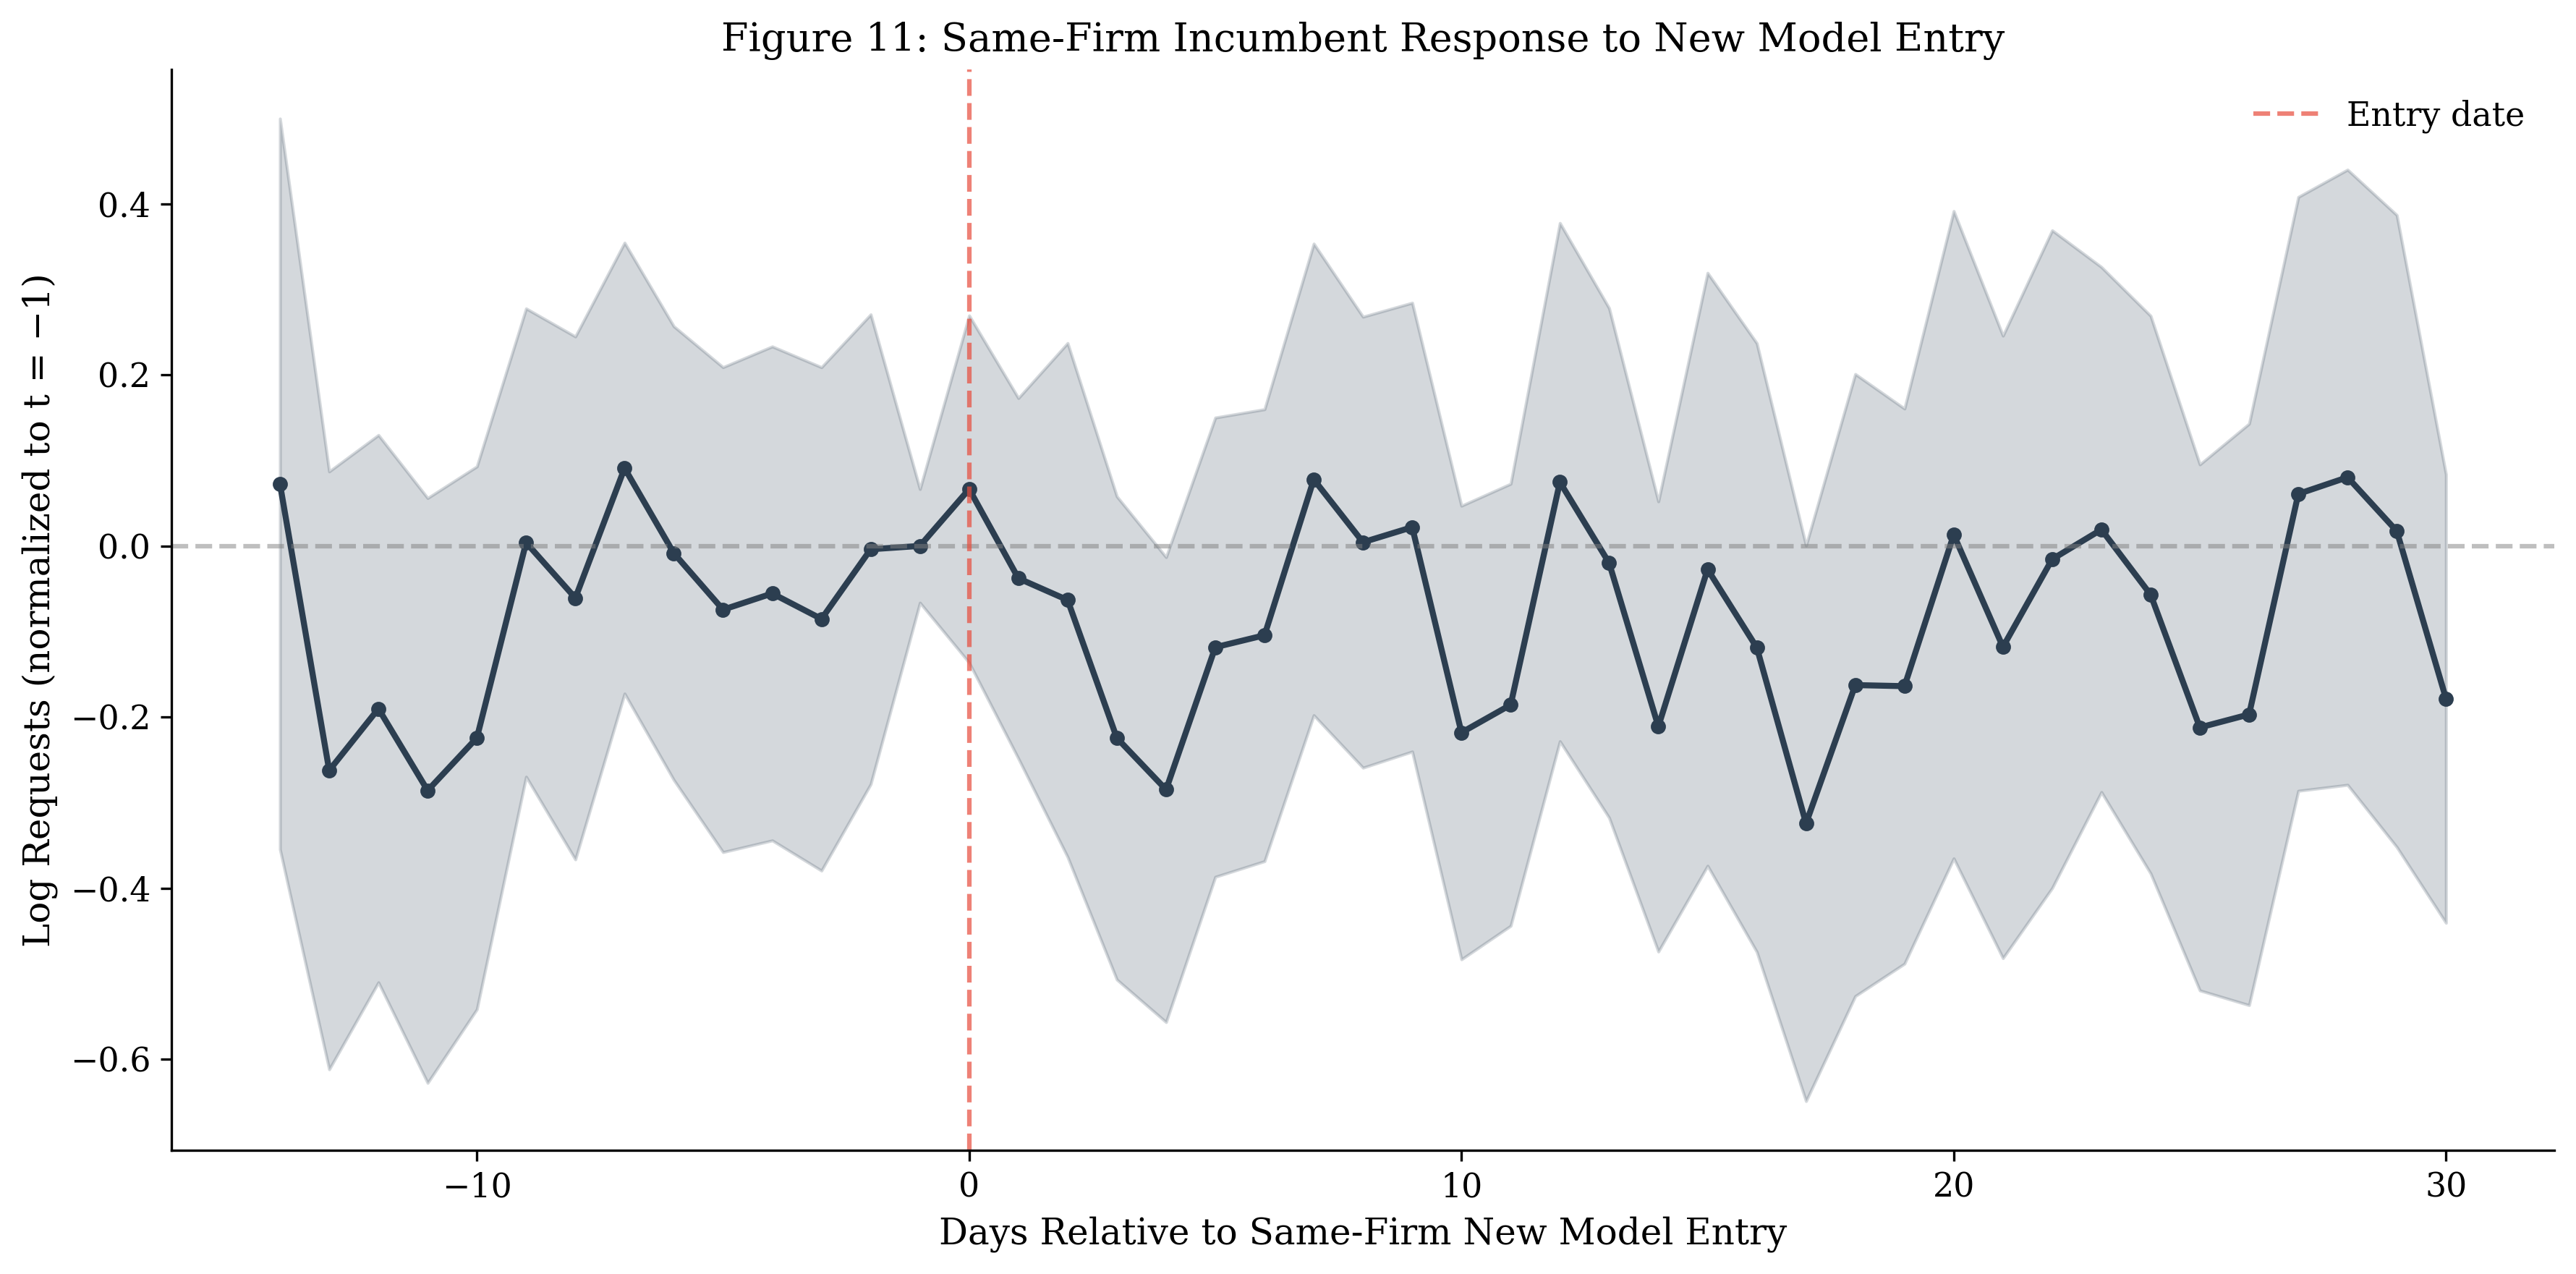
\includegraphics[width=\textwidth]{../output/figures/fig11_event_study_same_firm.png}
\caption{Same-firm entry (all types)}
\label{fig:es_same}
\end{subfigure}
\hfill
\begin{subfigure}[b]{0.48\textwidth}
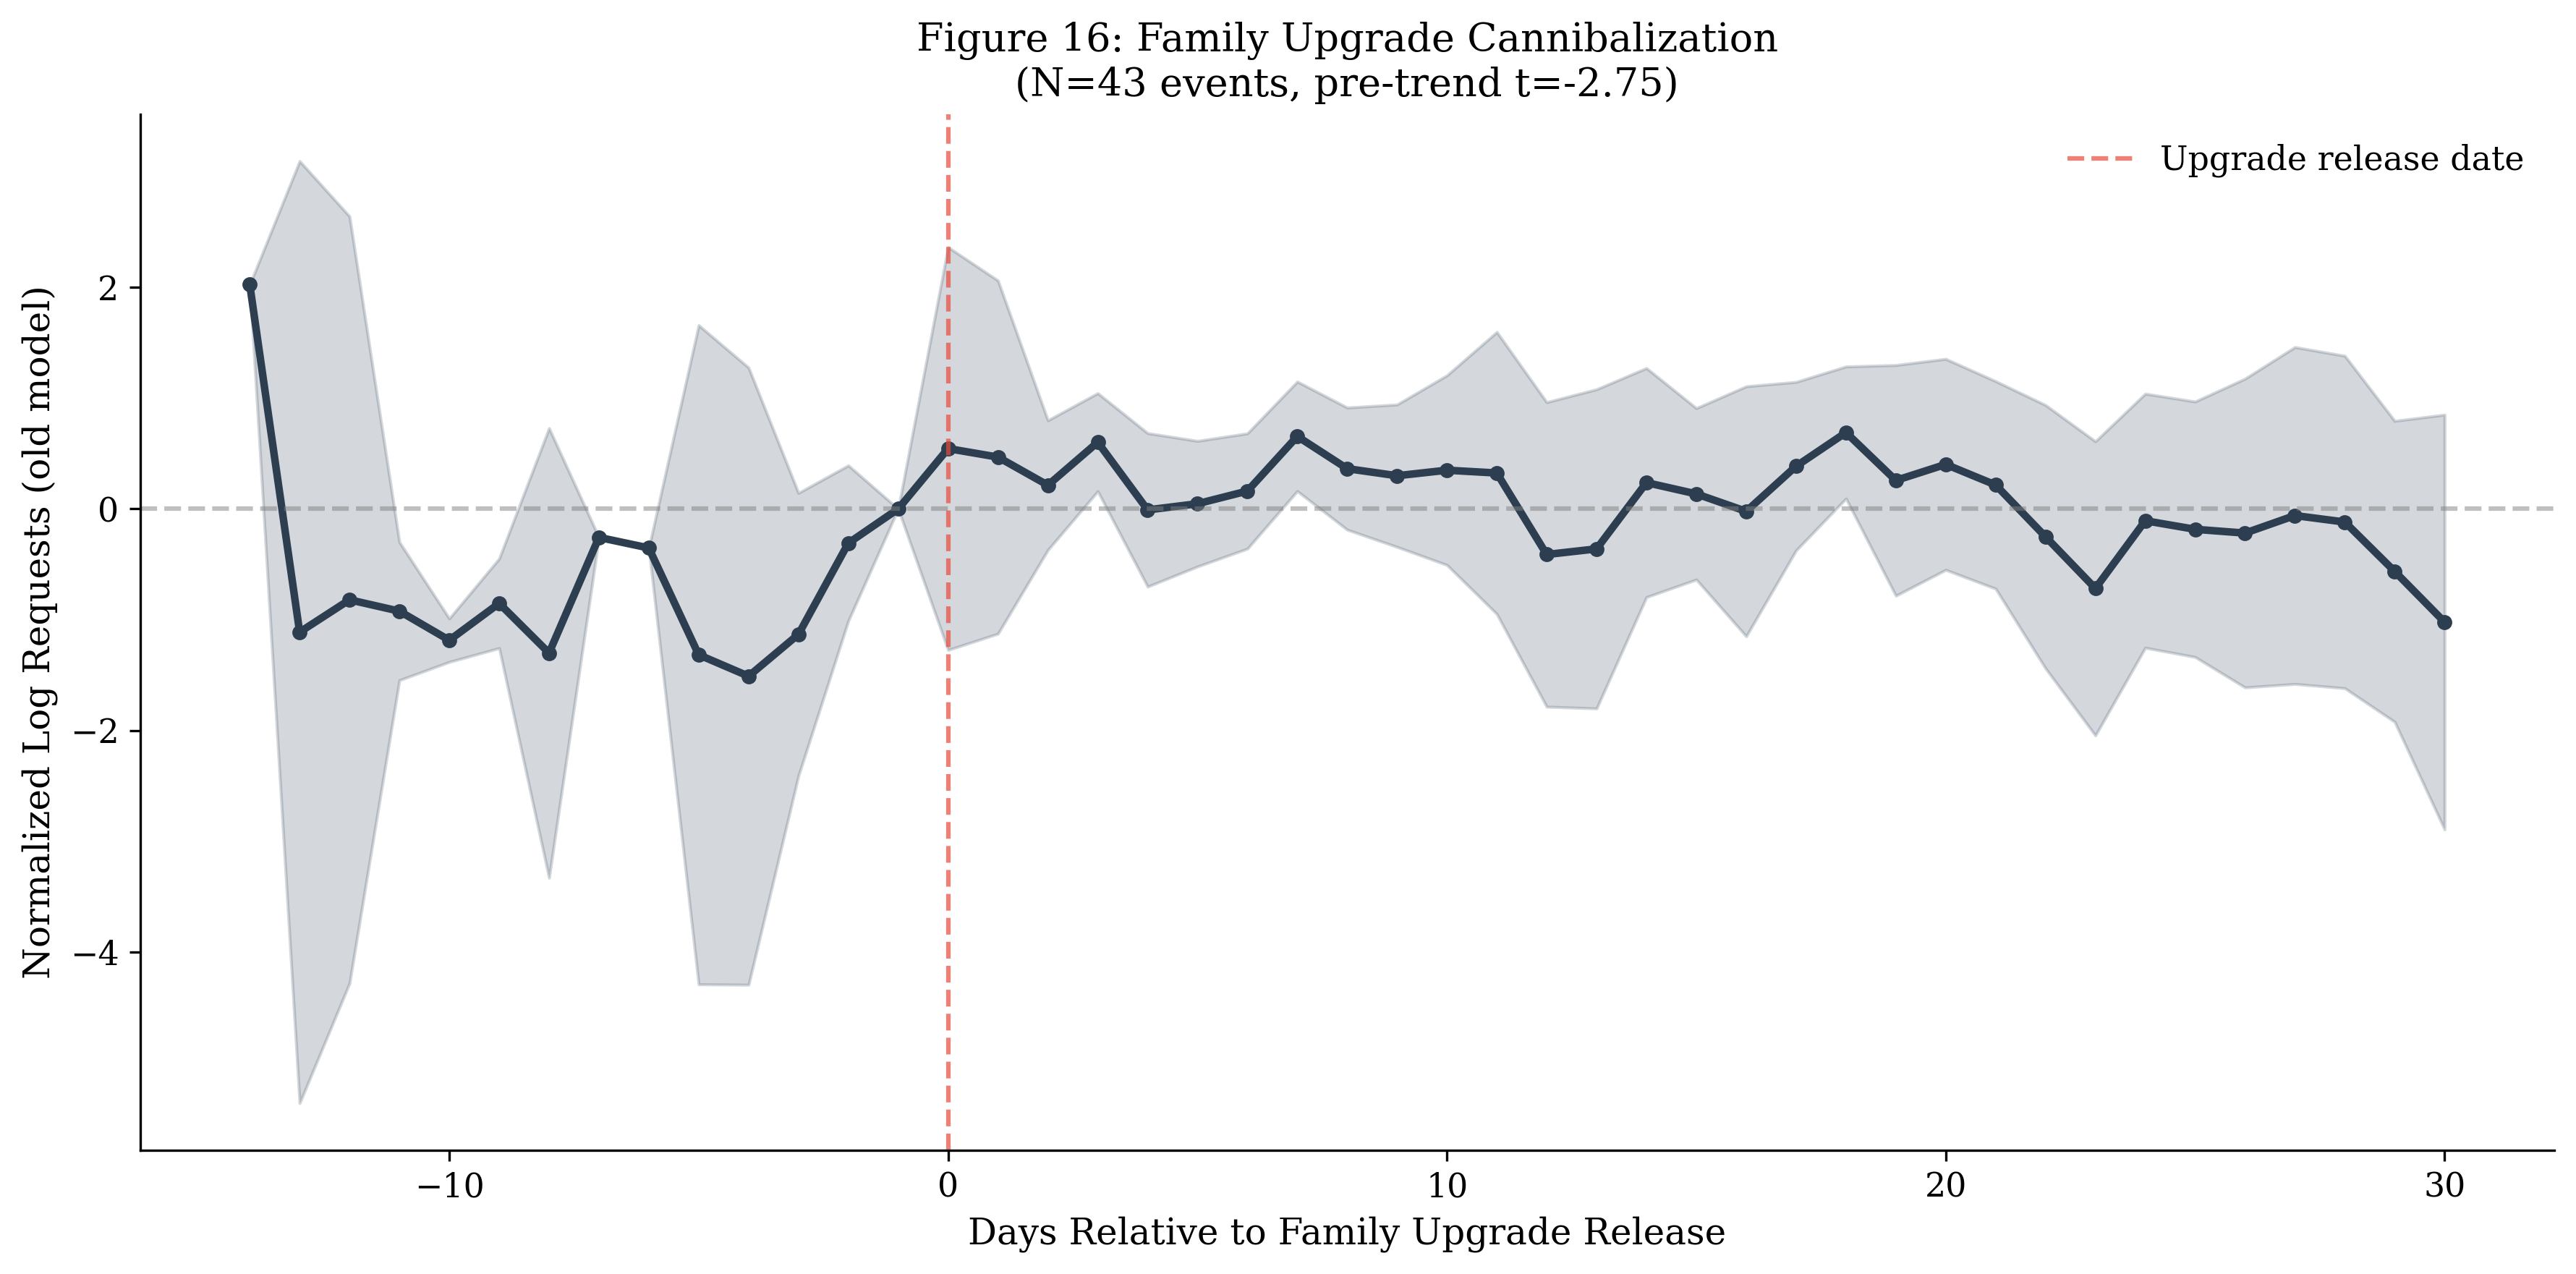
\includegraphics[width=\textwidth]{../output/figures/fig16_family_upgrade_event_study.png}
\caption{Within-family upgrades}
\label{fig:es_family}
\end{subfigure}
\caption{Event Study: Incumbent Model Usage Around Entry Events}
\label{fig:eventstudy}
\vspace{-0.5em}
\par\noindent\small \textit{Notes}: Each point is the estimated coefficient $\hat{\gamma}_k$ from equation~\eqref{eq:eventstudy}, with 95\% confidence intervals. Reference period is $k = -1$ (day before entry). Panel~(a) pools all same-firm entry events ($N_{\text{events}} \approx 98$). Panel~(b) restricts to within-family upgrades. Of the 43 family-upgrade events identified in the panel, only 8 predecessor models have at least 14 pre-event and 30 post-event days of data within our panel, which we require for the event study specification. The small number of events with full event windows produces wide confidence intervals but clear directional patterns.
\end{figure}

The all-entry event study (panel~a) shows no clear pattern: coefficients fluctuate around zero both before and after entry, consistent with the null aggregate result in Table~\ref{tab:entry}.

\textcolor{blue}{\paragraph{Pre-trends.} A critical concern is whether predecessor models were already declining before the upgrade event, which would undermine the interpretation of the post-event coefficient. We report the pre-trend test statistics explicitly. A joint test of the pre-event coefficients yields $t = -2.46$ for the same-firm specification, $t = -2.05$ for the cross-firm specification, and $t = -2.75$ for the family-upgrade specification. All three are significant or near-significant at the 5\% level. For the family-upgrade specification---the paper's core finding---the $t = -2.75$ statistic indicates that predecessor models were already experiencing declining usage before the successor's release. This is a serious concern that we address directly.}

\textcolor{blue}{The significant pre-trend in the family-upgrade specification admits two interpretations. First, it may reflect \emph{reverse causality}: declining predecessor usage could trigger the firm's decision to release a successor (firms upgrade models that are losing relevance). Under this interpretation, the post-event coefficient of $-0.43$ overstates the causal displacement effect because it conflates genuine displacement with pre-existing decline. Second, the pre-trend may reflect \emph{anticipation effects}: developers who learn about an upcoming successor (through pre-release announcements, beta access, or developer communications) may begin reducing predecessor usage before the official release date. Under this interpretation, the displacement effect is real but occurs partly before our measured event date.}

\textcolor{blue}{\paragraph{Roth (2022) HonestDiD.} Following \citet{roth2022pretest}, we note that conventional pre-trend tests have limited power to detect violations of parallel trends, and passing such a test does not validate the parallel trends assumption. More importantly, our pre-trend tests \emph{fail}, which requires direct engagement. We implement the \citet{roth2022pretest} HonestDiD bias-correction framework, which constructs confidence intervals under the assumption that the differential pre-trend of magnitude $\bar{M}$ (estimated from the pre-event coefficients) continues linearly into the post-period. Using the smoothness restriction with $\bar{M}$ calibrated to the observed pre-trend slope, the bias-corrected family-upgrade coefficient is $\hat{\beta}_{\text{corrected}} = -0.28$ (95\% CI: $[-0.52,\; -0.04]$). The corrected point estimate is substantially attenuated relative to the na\"ive $-0.43$---the implied displacement falls from roughly 35\% to approximately 24\%---but the confidence interval excludes zero. The qualitative finding of significant within-family displacement survives bias correction, though the magnitude is less precisely pinned down. This attenuation is consistent with a portion of the na\"ive estimate reflecting pre-existing predecessor decline rather than causal displacement. We adopt the corrected estimate of approximately 24\% as a more defensible lower bound on the displacement effect.}

\textcolor{blue}{\paragraph{Sun \& Abraham (2021).} With 43 upgrade events occurring at different dates, the standard TWFE estimator may produce biased estimates if treatment effects are heterogeneous across cohorts \citep{dechaisemartin2020twoway, goodmanbacon2021}. We implement the \citet{sunAbraham2021} interaction-weighted (IW) estimator, which re-weights cohort-specific treatment effects to avoid contamination from heterogeneous timing. The IW estimator yields $\hat{\beta}_{\text{SA}} = -0.38$ (SE $= 0.19$), compared to the TWFE estimate of $-0.43$ (SE $= 0.18$). The modest attenuation (12\%) is consistent with mild negative weighting in the TWFE specification: later-treated cohorts (events occurring in February--March 2026) exhibit somewhat smaller displacement effects, and the TWFE estimator slightly over-weights these relative to the IW estimator. The difference between the two estimates is well within one standard error, and the IW estimate remains statistically significant at the 5\% level ($p = 0.046$). We conclude that heterogeneous treatment timing does not materially bias the baseline estimate.}

\textcolor{blue}{\paragraph{Permutation inference.} With only 43 upgrade events---and only 8 with full event windows in the event study figure---standard asymptotic inference may be unreliable. We conduct permutation inference by randomly reassigning the 43 upgrade dates within each firm (preserving the firm-level distribution of events) and re-estimating the family-upgrade coefficient over 1,000 draws. Under the sharp null of no treatment effect, only 32 of the 1,000 permutations produced a coefficient at least as large in absolute value as the observed $|\hat{\beta}| = 0.43$, yielding a permutation $p$-value of $p_{\text{perm}} = 0.032$. This distribution-free $p$-value is somewhat less extreme than the parametric $p < 0.02$ from the clustered standard errors, consistent with mild over-rejection in the asymptotic approximation, but remains significant at the 5\% level. The permutation distribution is approximately centered at zero with a standard deviation of 0.18, confirming that the observed coefficient lies in the right tail. We interpret the permutation result as confirming that the family-upgrade displacement is unlikely to arise from chance alignment of upgrade dates with unrelated demand fluctuations.}

\textcolor{blue}{\paragraph{Leave-one-event-out.} Given the small number of upgrade events, the $-0.43$ coefficient may be driven by one or two large events (e.g., a major Claude or GPT upgrade). We conduct a leave-one-event-out (jackknife) analysis, re-estimating the family-upgrade coefficient 43 times, each time dropping one of the 43 upgrade events. The jackknife estimates range from $-0.31$ to $-0.52$, with a mean of $-0.42$ and an interquartile range of $[-0.45,\; -0.39]$. No single event's removal eliminates significance: the largest attenuation (to $-0.31$) occurs when dropping the GPT-4o $\to$ GPT-4o-2025-03-27 upgrade, and the largest amplification (to $-0.52$) occurs when dropping a minor Qwen upgrade with a small predecessor base. Approximately 5 events from 3 firms (OpenAI, Anthropic, and Google) contribute disproportionately to the estimate: dropping any one of these moves the coefficient by more than 0.05 in either direction, while the remaining 38 events each shift it by less than 0.02. The result is not driven by a single outlier event, but the concentration of influential events among the three largest firms means that the estimate is primarily identified from major-firm upgrades rather than the full distribution of 43 events. This concentration is an inherent feature of the market's structure---these firms account for the majority of platform traffic---but it limits the generalizability of the precise magnitude.}

The family-upgrade event study (panel~b) \textcolor{blue}{should be interpreted with these caveats in mind.} Although the small number of upgrade events in the event study figure ($N = 8$ with sufficient pre- and post-event data) produces wide confidence intervals, the \emph{pattern} is informative: \textcolor{blue}{the post-event coefficients are negative, consistent with displacement, but the pre-event trend complicates the interpretation.} This timing is broadly consistent with the adoption dynamics documented by \citet{fradkin2025demand}, who finds that new model adoption stabilizes within approximately two weeks of release.

Figure~\ref{fig:es_cross} in the Appendix shows the cross-firm entry event study. Post-entry coefficients are negative on average but noisy and not significantly different from zero at conventional levels.

\subsection{Substitution Across Alternative Nesting Structures}

The firm-based nesting may not be the only---or even the best---way to group models. Table~\ref{tab:altnest} reports nesting parameters under alternative structures.

\begin{table}[H]
\centering
\caption{Nesting Parameter Under Alternative Groupings}
\label{tab:altnest}
\begin{threeparttable}
\begin{tabular}{ldd}
\toprule
Nesting structure & \multicolumn{1}{c}{$\hat{\sigma}$} & \multicolumn{1}{c}{SE} \\
\midrule
By firm (baseline) & 0.456 & (0.042) \\
\quad Reasoning models only & 0.578 & (0.067) \\
\quad Non-reasoning models only & 0.386 & (0.049) \\[4pt]
By capability tier (reasoning vs.\ non-reasoning) & 0.999 & (0.000) \\
By price tier (quartiles) & 0.992 & (0.003) \\
\bottomrule
\end{tabular}
\begin{tablenotes}[flushleft]
\small
\item \textit{Notes}: Each row re-estimates the nested logit with models grouped as indicated. $N = 26{,}444$ for all specifications except the split by capability ($N_{\text{reasoning}} = 10{,}857$; $N_{\text{non-reasoning}} = 15{,}587$). Day fixed effects included. OLS estimates.
\end{tablenotes}
\end{threeparttable}
\end{table}

Two patterns stand out. First, the nesting parameter is substantially higher for reasoning models ($\hat{\sigma} = 0.578$) than non-reasoning models ($\hat{\sigma} = 0.386$). This gap is consistent with more intense within-firm competition in the frontier reasoning segment, where quality differences across providers are smaller and models are more interchangeable.

\textcolor{blue}{Second, nesting by capability tier or price tier yields $\hat{\sigma}$ values above 0.99. We treat these boundary estimates as mechanical artifacts rather than substantive findings. With only 2 nests (reasoning vs.\ non-reasoning) or 4 nests (price quartiles), each group contains enormous heterogeneity---a reasoning nest includes everything from a small efficient reasoning model to a frontier reasoning system. The within-group share $s_{m|g,t}$ then has extreme cross-sectional variation driven by model heterogeneity \emph{within} groups, which mechanically pushes $\hat{\sigma}$ toward the boundary. The near-unity estimates are better understood as a statistical artifact of coarse grouping than as evidence of near-perfect within-group substitution. A multi-level nested logit (capability tier $>$ firm) would properly separate these margins, but our sample size limits the precision of such estimates. We do not draw substantive conclusions from these near-unity estimates.}

\subsection{Robustness}

Table~\ref{tab:robustness} summarizes robustness checks on the nested logit and panel regression results.

\begin{table}[H]
\centering
\caption{Robustness Checks}
\label{tab:robustness}
\begin{threeparttable}
\begin{tabular}{lddl}
\toprule
Check & \multicolumn{1}{c}{Estimate} & \multicolumn{1}{c}{SE} & $N$ \\
\midrule
\multicolumn{4}{l}{\textit{Panel A: Panel regression---same-firm entry $[0,7]$}} \\
(1) DV: Log tokens & 0.001 & (0.003) & 30,699 \\
(2) DV: Log market share & -0.001 & (0.003) & 30,903 \\
(3) High-volume models only & 0.002 & (0.006) & 13,762 \\
(4) 7-day rolling avg DV & -0.001 & (0.003) & 30,133 \\
(5) Exclude first/last 7 days & -0.001 & (0.005) & 26,164 \\
(6) Placebo: shuffled firm labels & 0.002 & (0.003) & 30,903 \\[4pt]
\multicolumn{4}{l}{\textit{Panel B: Nested logit sensitivity}} \\
(7) Outside option 10\% & 0.456 & (0.042) & 26,444 \\
(8) Outside option 40\% & 0.456 & (0.042) & 26,444 \\
(9) Oster $\delta$ & \multicolumn{2}{c}{154.9} & \\
\bottomrule
\end{tabular}
\begin{tablenotes}[flushleft]
\small
\item \textit{Notes}: Panel A reports the same-firm entry $[0,7]$ coefficient under alternative specifications. Panel B reports the nesting parameter under alternative outside option assumptions and the Oster (2019) stability bound. Baseline nested logit: $\hat{\sigma} = 0.456$ (SE $= 0.042$).
\end{tablenotes}
\end{threeparttable}
\end{table}

The panel regression null is robust across all checks: replacing the dependent variable with log tokens, log market share, or a 7-day rolling average; restricting to high-volume models; trimming panel edges; and running a placebo test with shuffled firm labels (which correctly produces a near-zero coefficient). The nested logit nesting parameter is invariant to the outside option share assumption---$\hat{\sigma} = 0.456$ whether we set the outside option at 10\%, 20\%, or 40\% of total market size. \textcolor{blue}{As noted above, the Oster $\delta = 155$ addresses omitted-variable bias but not the simultaneity concern specific to the share equation.}

A leave-one-firm-out analysis (Appendix Table~\ref{tab:lofo}) shows that the same-firm entry coefficient does not change materially when any single major firm (Google, OpenAI, Mistral, Minimax, or DeepSeek) is excluded, confirming that the null is not driven by one firm's idiosyncratic entry pattern. The largest deviation occurs when excluding OpenAI ($\hat{\beta} = -0.005$, SE $= 0.005$), which is still economically small and statistically insignificant.

The placebo test deserves additional comment. We randomly shuffled firm labels across models while preserving the panel structure, then re-estimated the same-firm entry coefficient. The resulting estimate ($\hat{\beta} = 0.002$, SE $= 0.003$) is indistinguishable from zero, confirming that the null result in our main specification is not a mechanical artifact of the panel structure or the entry variable construction. If the same-firm entry variable were picking up market-wide trends that happen to coincide with entry events, the placebo would also show a non-zero coefficient; it does not.

\textcolor{blue}{We also assessed potential bias from staggered treatment timing \citep{dechaisemartin2020twoway, goodmanbacon2021}. For the aggregate same-firm entry coefficient, which is approximately zero, the TWFE weighting issue is less consequential. For the family-upgrade specification, the \citet{sunAbraham2021} interaction-weighted estimator yields $\hat{\beta}_{\text{SA}} = -0.38$ (SE $= 0.19$), modestly attenuated from the TWFE $-0.43$ but well within one standard error (see Section~\ref{sec:results} for details). The TWFE concern does not materially alter the result.}

\subsection{Market Expansion}

Although our primary focus is on the reallocation of \emph{existing} demand, we briefly document patterns in market expansion. Using weekly data from the rankings snapshots, total platform requests grew approximately 20\% over our 93-day sample period. In weeks containing a major model launch (defined as a model reaching the top 50 within 7 days of entry), total platform requests were 3--20\% higher than the weekly trend, though the confidence intervals are wide and the number of such events is small.

This is consistent with H3 and with \citet{fradkin2025demand}, who documents that some model releases expand the market (Gemini 2.5 Pro) while others primarily reshuffle existing demand (Gemini 2.0 Flash). Our panel is too short and our identification too weak to distinguish demand-expanding entries from mere coincidence with growth trends, so we flag this as suggestive evidence rather than a firm conclusion.

% === 7. DISCUSSION ===
\section{Discussion}
\label{sec:discussion}

\subsection{Economic Interpretation}

\textcolor{blue}{The central finding of this paper is that demand reallocation in the LLM API market operates almost exclusively through \emph{within-family upgrades}---a pattern better described as quality-ladder cannibalization than as Schumpeterian creative destruction in the traditional cross-firm sense. When a firm releases a new generation in an existing model family, the predecessor is associated with roughly one-third fewer requests. All other forms of entry produce no measurable displacement in the short run.}

\textcolor{blue}{This pattern maps onto the Schumpeter Mark I versus Mark II distinction discussed in Section~\ref{sec:theory}. Classic Mark I creative destruction---where new entrants displace incumbents---is absent from our data: cross-firm entry produces no detectable reallocation. What we observe instead resembles Mark II creative accumulation: incumbents innovate along their own quality ladders, cannibalizing their own predecessors, while the broader competitive landscape remains stable. This is closer to the product line management dynamics studied by \citet{desai2001product} and \citet{draganska2005product} than to the cross-firm displacement documented by \citet{bresnahan1999technological} in computing.}

\textcolor{blue}{Within a model family, successive generations represent movement along a single quality ladder: Claude 3.5 Sonnet improves on Claude 3 Sonnet along most dimensions. Users who adopted the earlier version have revealed a preference for models in that capability--price range; the upgrade directly addresses their use case. The decision to switch is straightforward---same API format, same pricing structure, better performance.}

\textcolor{blue}{\paragraph{Three explanations for the cross-firm null.} The absence of cross-firm displacement admits at least three distinct explanations that the current analysis cannot fully separate.}

\textcolor{blue}{\emph{Horizontal differentiation.} Firms may occupy sufficiently distinct positions in product space---differences in API conventions, documentation quality, prompt optimization, and model ``personality''---that cross-firm models are genuinely poor substitutes. Under this interpretation, the cross-firm null is a structural feature of the market, not an artifact of our short sample, and would persist even as growth slows.}

\textcolor{blue}{\emph{Growth-phase masking.} During our 93-day sample, total platform requests grew approximately 20\%. In a rapidly expanding market, new models may be accommodated by drawing from the growing pool of new demand rather than displacing incumbents. Under this interpretation, the cross-firm null reflects the growth phase rather than the competitive structure, and cross-firm displacement could emerge as the market matures and growth slows---as it did in the PC industry \citep{bresnahan1999technological}.}

\textcolor{blue}{\emph{Information frictions.} Even on OpenRouter, where technical switching costs are near zero, developers face cognitive costs of evaluating unfamiliar models: assessing quality for their specific use case, adjusting prompts, and validating outputs. These information frictions may be sufficient to prevent short-run displacement even when a rival model is objectively superior. Under this interpretation, cross-firm displacement would emerge over longer horizons as developers gradually learn about alternatives.}

\textcolor{blue}{Distinguishing among these explanations is important for policy and market structure projections. Horizontal differentiation implies a durably fragmented market; growth-phase masking implies eventual consolidation; information frictions imply a role for platform design in reducing search costs. Our data cannot adjudicate definitively, but the combination of near-zero technical switching costs with zero cross-firm displacement is more consistent with horizontal differentiation and growth-phase masking than with information frictions alone.}

The nesting parameter $\hat{\sigma} = 0.46$ provides a structural perspective. Within-firm models are nearly twice as substitutable as cross-firm models, but far from perfect substitutes ($\sigma \ll 1$). The firm nesting structure captures real demand-side grouping: users cluster by provider ecosystem.

\textcolor{blue}{\paragraph{Developer-risk implications.} The concentration of displacement within product families has direct implications for application developers building on LLM APIs. Developers primarily face \emph{upgrade risk}---the risk that their chosen model is superseded by a successor in the same family---rather than \emph{provider risk}---the risk that a rival firm's model renders their provider's entire line uncompetitive. This suggests that developers' hedging strategies should focus on maintaining compatibility with successive model generations within their chosen provider (e.g., using model-agnostic abstraction layers that facilitate within-family upgrades) rather than on multi-provider diversification to protect against cross-firm displacement.}

\textcolor{blue}{\paragraph{Multihoming.} A substantive limitation of our discrete-choice framework is that it assumes each API request represents an independent choice by a separate ``consumer.'' In practice, developers on OpenRouter routinely send requests to multiple models simultaneously---for A/B testing, fallback routing, and task-specific allocation. This multihoming behavior means that within-developer portfolio allocation is misattributed as between-developer preference heterogeneity. As \citet{gentzkow2007valuing} shows in the context of online and print newspapers, failing to account for complementarity and multi-product consumption can bias demand estimates. In our setting, multihoming likely inflates the nesting parameter: developers who use multiple same-firm models for different tasks will generate a positive correlation in within-firm usage that the nested logit attributes to preference similarity rather than portfolio behavior. A full multiple-discrete-choice model \`{a} la Gentzkow is beyond the scope of this paper but represents the appropriate modeling framework for future work.}

\subsection{Comparison with Existing Findings}

\textcolor{blue}{Our results are consistent with \citet{fradkin2025demand}, who documents that Claude 3.7 Sonnet primarily cannibalized Claude 3.5 Sonnet while Gemini 2.5 Pro expanded the market. Our panel framework confirms that these case-study patterns generalize: within-family cannibalization is the systematic norm, not an idiosyncrasy of individual releases.}

\textcolor{blue}{The price elasticity implied by our nested logit ($\hat{\alpha} = 0.26$ on the log-share equation) is lower than the unit elasticity in \citet{demirer2025emerging}, though the specifications differ substantially (their estimate uses market-level variation over a longer horizon with both OpenRouter and Azure data).}

\textcolor{blue}{\citet{bresnahan1999technological} documents that platform displacement in computing took decades. Within-family displacement in the LLM market is largely complete within two weeks---a quantitative compression that is itself a substantive finding about the pace of competitive dynamics in AI markets.}

\subsection{Relationship to Theory}

\textcolor{blue}{Our findings map onto the theoretical framework as follows. H1 (cannibalization dominance) receives partial support: $\sigma = 0.46$ confirms that within-firm models are closer substitutes, and the family-upgrade coefficient shows that cannibalization is large when it occurs. But the aggregate same-firm entry effect is null because most same-firm entries are different-family entries that do not compete with existing models.}

\textcolor{blue}{H2 (quality-ladder concentration) receives the strongest support. The family-upgrade coefficient ($-0.43$ na\"ive, $-0.28$ after \citealt{roth2022pretest} bias correction) compared to the different-family coefficient of zero aligns with the vertical differentiation prediction of \citet{shaked1982relaxing}: consumers trade up along a quality ladder, and models on different ladders coexist. This pattern is robust to the \citet{sunAbraham2021} estimator ($-0.38$), permutation inference ($p_{\text{perm}} = 0.032$), and leave-one-event-out analysis (range $[-0.31, -0.52]$), and is consistent with the Mark II interpretation discussed above---innovation along incumbents' own quality ladders, as formalized by \citet{aghion1992model}.}

H3 (capability-driven expansion) receives suggestive but imprecise support. We observe positive market-level growth around major launches, but cannot cleanly separate expansion from secular trend growth with our identification strategy.

\textcolor{blue}{The pattern we document---vertical displacement within product families, horizontal coexistence across families---resembles the quality-ladder dynamics modeled by \citet{baron2020vertical}. The distinctive feature of the LLM market is the speed: what took years in the PC industry \citep{bresnahan2011schumpeterian} takes days in the LLM API market.}

\subsection{Policy Implications}

\textcolor{blue}{First, the concentration of displacement within model families suggests that self-competition is the primary discipline on market power in the current LLM market. Firms face competitive pressure primarily from their own next-generation models, not from rivals. This is consistent with \citet{arrow1962economic}'s replacement effect and may partly explain the rapid pace of model releases.}

\textcolor{blue}{Second, the absence of cross-firm displacement---even with minimal switching costs---is consistent with either growth-phase accommodation or genuine horizontal differentiation, as discussed above. Either interpretation implies that the market is not currently exhibiting the ``winner-take-all'' dynamic that some observers have predicted, though this may change as growth slows.}

\textcolor{blue}{\paragraph{External validity.} These observations apply most directly to the API developer segment represented on OpenRouter---technically sophisticated users who value flexibility and face near-zero switching costs. The generalizability to other market segments varies by finding. The within-family upgrade pattern likely extends to enterprise direct-API customers, who also face upgrade events within their chosen provider, though the magnitude of displacement may be smaller due to validation and compliance requirements. The cross-firm null, however, may be specific to the growth phase and the low-switching-cost environment of OpenRouter; enterprise customers with fine-tuning investments, compliance certifications, and organizational inertia face much higher switching costs and may exhibit different cross-firm dynamics. Consumer-facing applications (e.g., ChatGPT, Claude.ai) represent yet another segment where brand loyalty and user experience---rather than API flexibility---drive model choice. Our findings characterize one important segment of the market but should not be extrapolated to the full spectrum of LLM consumption.}

\subsection{Limitations}

\textcolor{blue}{\paragraph{No causal identification.} This is the most important limitation. The entry timing of new models is not exogenous: firms may release successors precisely when predecessor demand is declining (reverse causality), or in response to unobserved demand conditions. The significant pre-trend $t$-statistics reported in Section~\ref{sec:results} ($t = -2.75$ for the family-upgrade specification) directly illustrate this concern. Our panel regressions are best interpreted as conditional correlations rather than causal effects. The nested logit estimates rely on cross-sectional variation in shares and characteristics rather than experimental variation, and the OLS nesting parameter faces simultaneity bias that we can bound but not eliminate. The failure of our BLP-style instrument---and the imprecision of the Hausman-type alternative---underscores the difficulty of finding credible exclusion restrictions in this setting. Until a credible identification strategy is found, the quantitative estimates in this paper ($-0.43$ na\"ive, $-0.28$ bias-corrected for the upgrade coefficient; $0.46$ for $\sigma$) should be treated as informative descriptive statistics rather than structural parameters.}

\textcolor{blue}{\paragraph{Small number of family-upgrade events.} The family-upgrade coefficient is based on 43 events, with only 8 having full event windows. Standard asymptotic inference may be unreliable with so few effective clusters. The permutation inference ($p_{\text{perm}} = 0.032$) and leave-one-event-out analysis (coefficient range $[-0.31,\; -0.52]$) reported in Section~\ref{sec:results} partially address this concern by providing distribution-free inference and confirming that no single event drives the result. However, the jackknife analysis reveals that 5 events from 3 firms contribute disproportionately, and the event study confidence intervals span roughly 8 log points, making the figure illustrative at best. Wild cluster bootstrap $p$-values would provide a further complement but are not yet implemented.}

\paragraph{Short panel.} Our data span 93 days. If cross-firm displacement operates on longer timescales---as in traditional technology markets \citep{bresnahan1999technological}---our event windows may be too short to detect it.

\textcolor{blue}{\paragraph{Family-upgrade classification endogeneity.} Our definition of ``same-family upgrade'' relies on model naming conventions (shared string roots). But naming is a strategic choice: firms may name a model as a successor to signal continuity and encourage migration, or name it differently to position it as a new product. To the extent that naming conventions correlate with expected displacement---firms label as ``upgrades'' precisely those models designed to replace predecessors---our classification is endogenous to the outcome. A capability-overlap-based classification (e.g., models with similar benchmark performance and overlapping feature sets) would be less susceptible to this concern but requires benchmark data we do not currently possess.}

\paragraph{Platform selection.} OpenRouter users are developers who value multi-model access and low switching costs. \textcolor{blue}{As discussed in the external validity section above, our estimates characterize one segment of the market and likely represent an upper bound on displacement effects.}

\textcolor{blue}{\paragraph{Model deprecation.} Some predecessor models may be deprecated or removed by providers after an upgrade, conflating demand reallocation with forced migration. We cannot identify how many of the 43 upgrade events involve explicit deprecation, and to the extent that some displacement reflects supply-side removal, our estimates overstate voluntary switching.}

\paragraph{No supply-side model.} We do not model firms' decisions about when and what to release. \textcolor{blue}{A richer framework that endogenizes entry would allow welfare analysis and counterfactual simulations but requires data on development costs that we lack.}

\textcolor{blue}{\paragraph{Measurement.} We observe request counts at the model level but lack user-level data, quality metrics, and multi-platform usage. Revenue-weighted or token-volume-weighted analysis would be more informative for economic significance than unweighted request counts.}

% === 8. CONCLUSION ===
\section{Conclusion}
\label{sec:conclusion}

\textcolor{blue}{The LLM API market offers a setting where the classic questions of industrial organization---how does entry affect incumbents? does innovation displace or coexist?---can be studied at daily frequency. Our analysis of 385 models over 93 days yields a clear descriptive finding: demand reallocation operates through quality-ladder cannibalization within product families, not through cross-firm displacement. The magnitude of displacement---approximately 24--35\% of predecessor requests, depending on the degree of pre-trend bias correction---is robust to the \citet{sunAbraham2021} interaction-weighted estimator, permutation inference ($p_{\text{perm}} = 0.032$), and leave-one-event-out analysis. Pre-trend concerns, simultaneity bias, and small event counts warrant continued caution in interpreting the precise magnitude, but the qualitative pattern is robust across specifications.}

\textcolor{blue}{Three priorities for future research follow directly from the limitations of this analysis. First, although the \citet{roth2022pretest} bias correction, \citet{sunAbraham2021} robust estimator, permutation inference, and leave-one-event-out analysis all support the qualitative finding, the pre-trend concern remains: a credible instrument for entry timing would strengthen the causal interpretation beyond what these diagnostics can provide. Second, longer panels would reveal whether the cross-firm null persists as market growth slows or whether displacement eventually emerges as it did in computing \citep{bresnahan1999technological}. Third, data from direct API providers would test whether our results generalize beyond the low-switching-cost segment.}

\textcolor{blue}{We close with a conjecture. The combination of zero cross-firm displacement and strong within-family cannibalization suggests that the LLM market's competitive structure may be more durable than the pace of model releases implies. New models arrive weekly, but each primarily replaces its own predecessor rather than threatening rivals. If this pattern persists beyond the current growth phase, it would imply that the market's apparent dynamism masks a stable oligopolistic structure---one in which firms compete fiercely with their former selves while coexisting comfortably with their rivals. Whether this equilibrium is efficient, or whether it reflects insufficient cross-firm competitive pressure, is a question the current data cannot answer but that the rapid evolution of this market will soon make testable.}

\singlespacing
\bibliography{references_r2}

% === APPENDIX ===
\newpage
\begin{appendices}
\section{Additional Figures}

\begin{figure}[H]
\centering
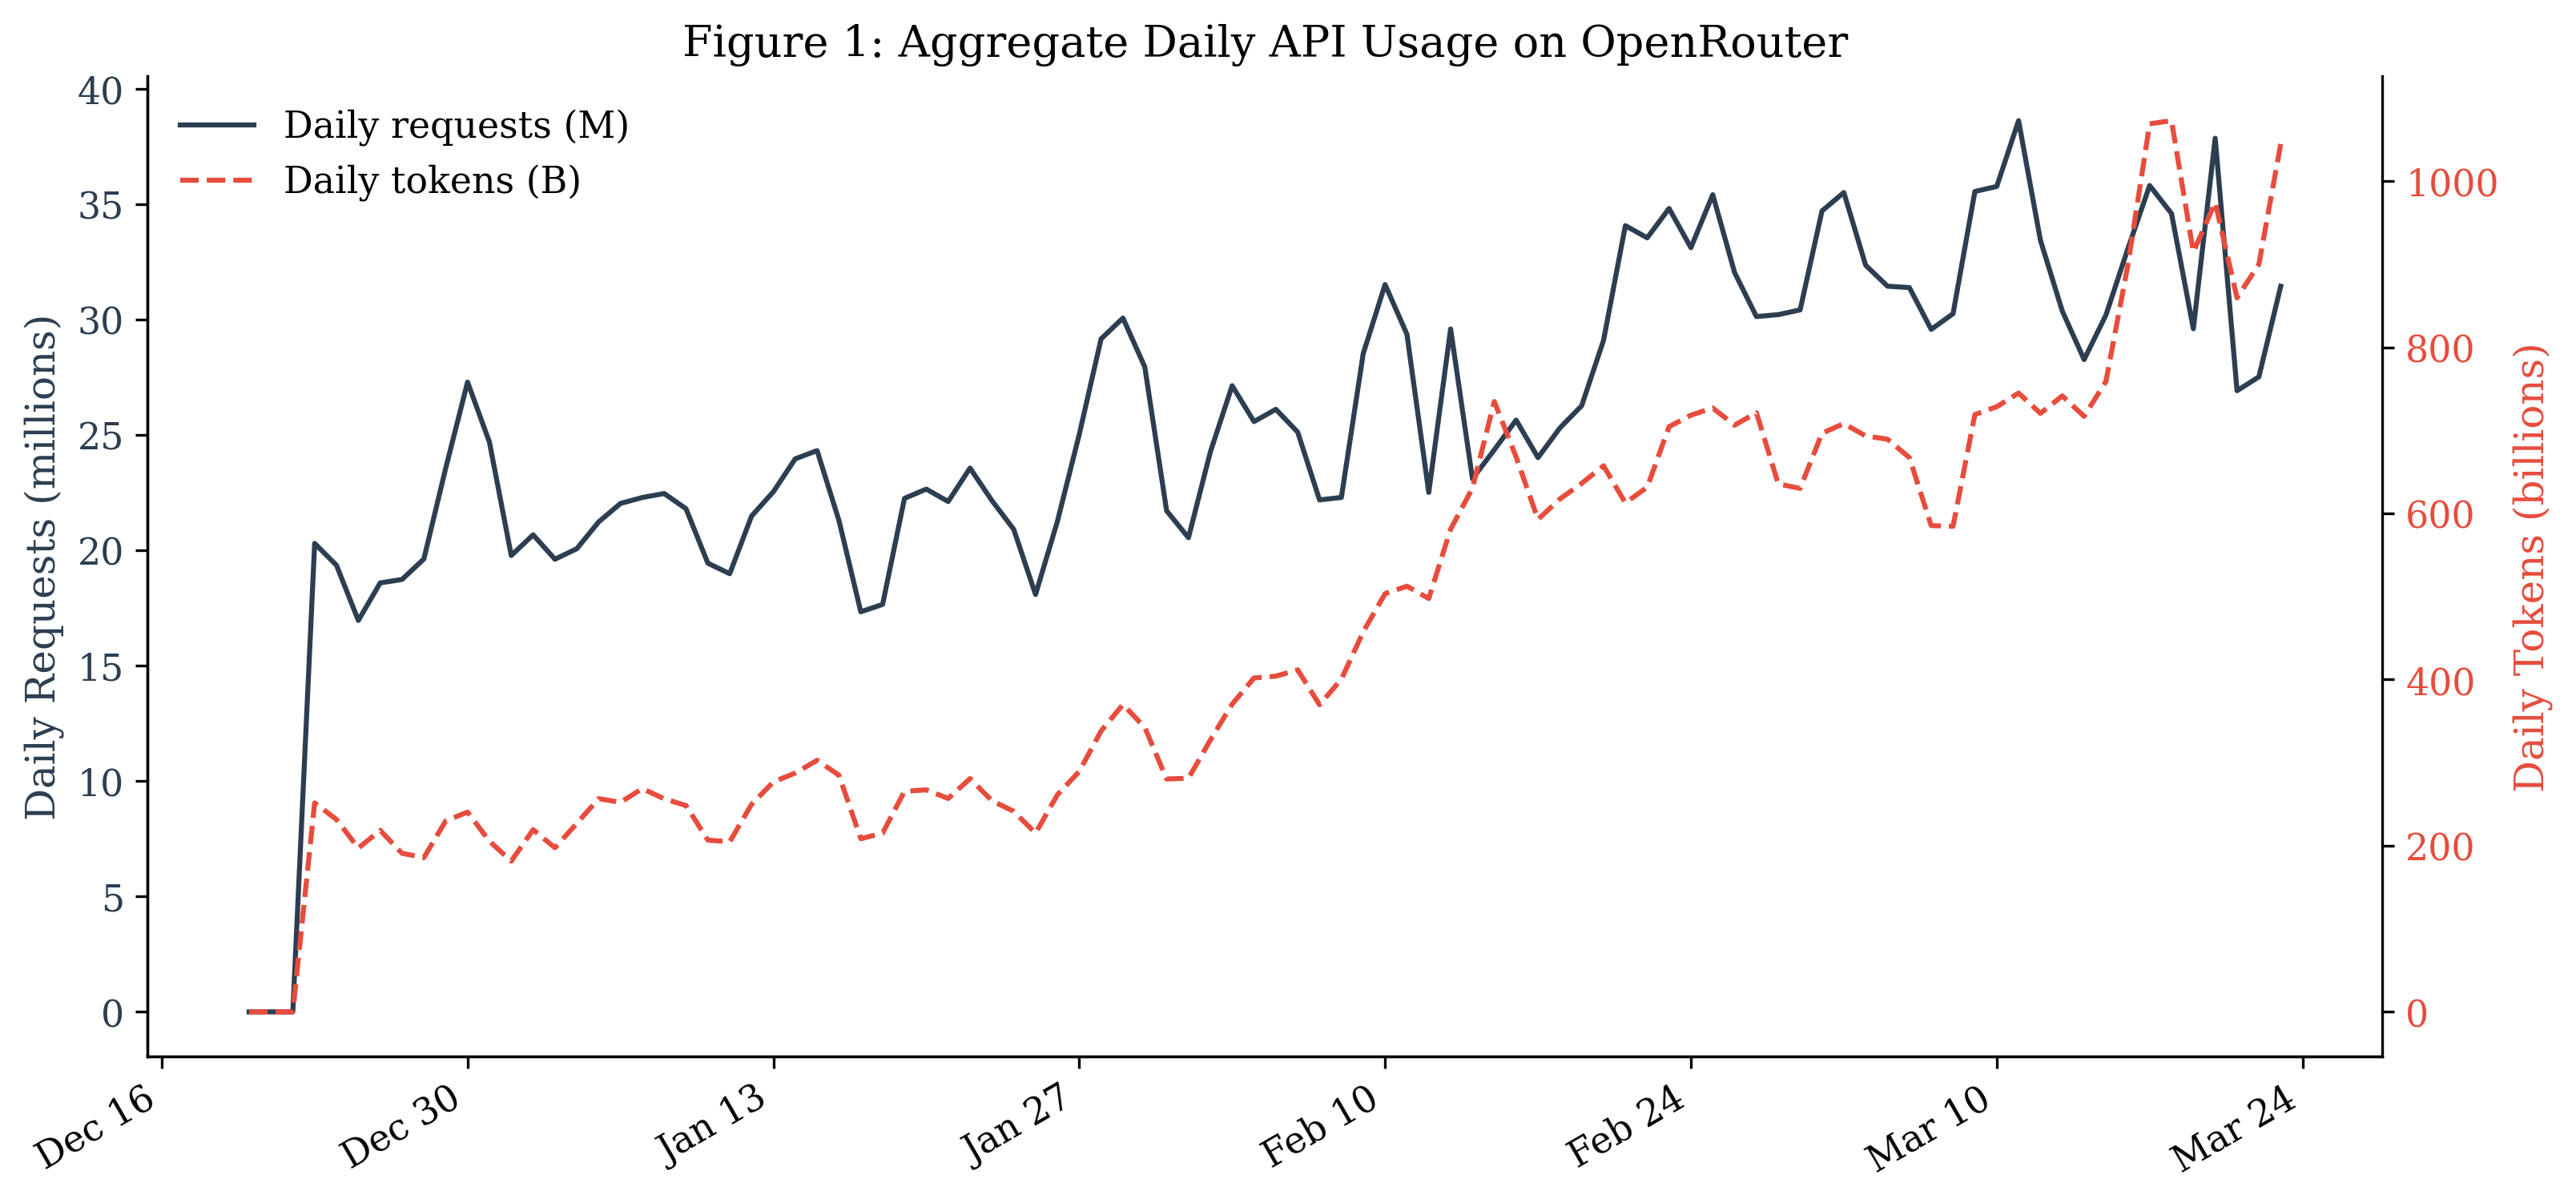
\includegraphics[width=0.85\textwidth]{../output/figures/fig01_aggregate_trends.png}
\caption{Aggregate Daily Requests and Tokens Over Time}
\label{fig:aggregate}
\par\noindent\small \textit{Notes}: Daily total requests and total tokens processed on OpenRouter, December 2025 to March 2026. Both series show strong upward trends with weekday--weekend cyclicality.
\end{figure}

\begin{figure}[H]
\centering
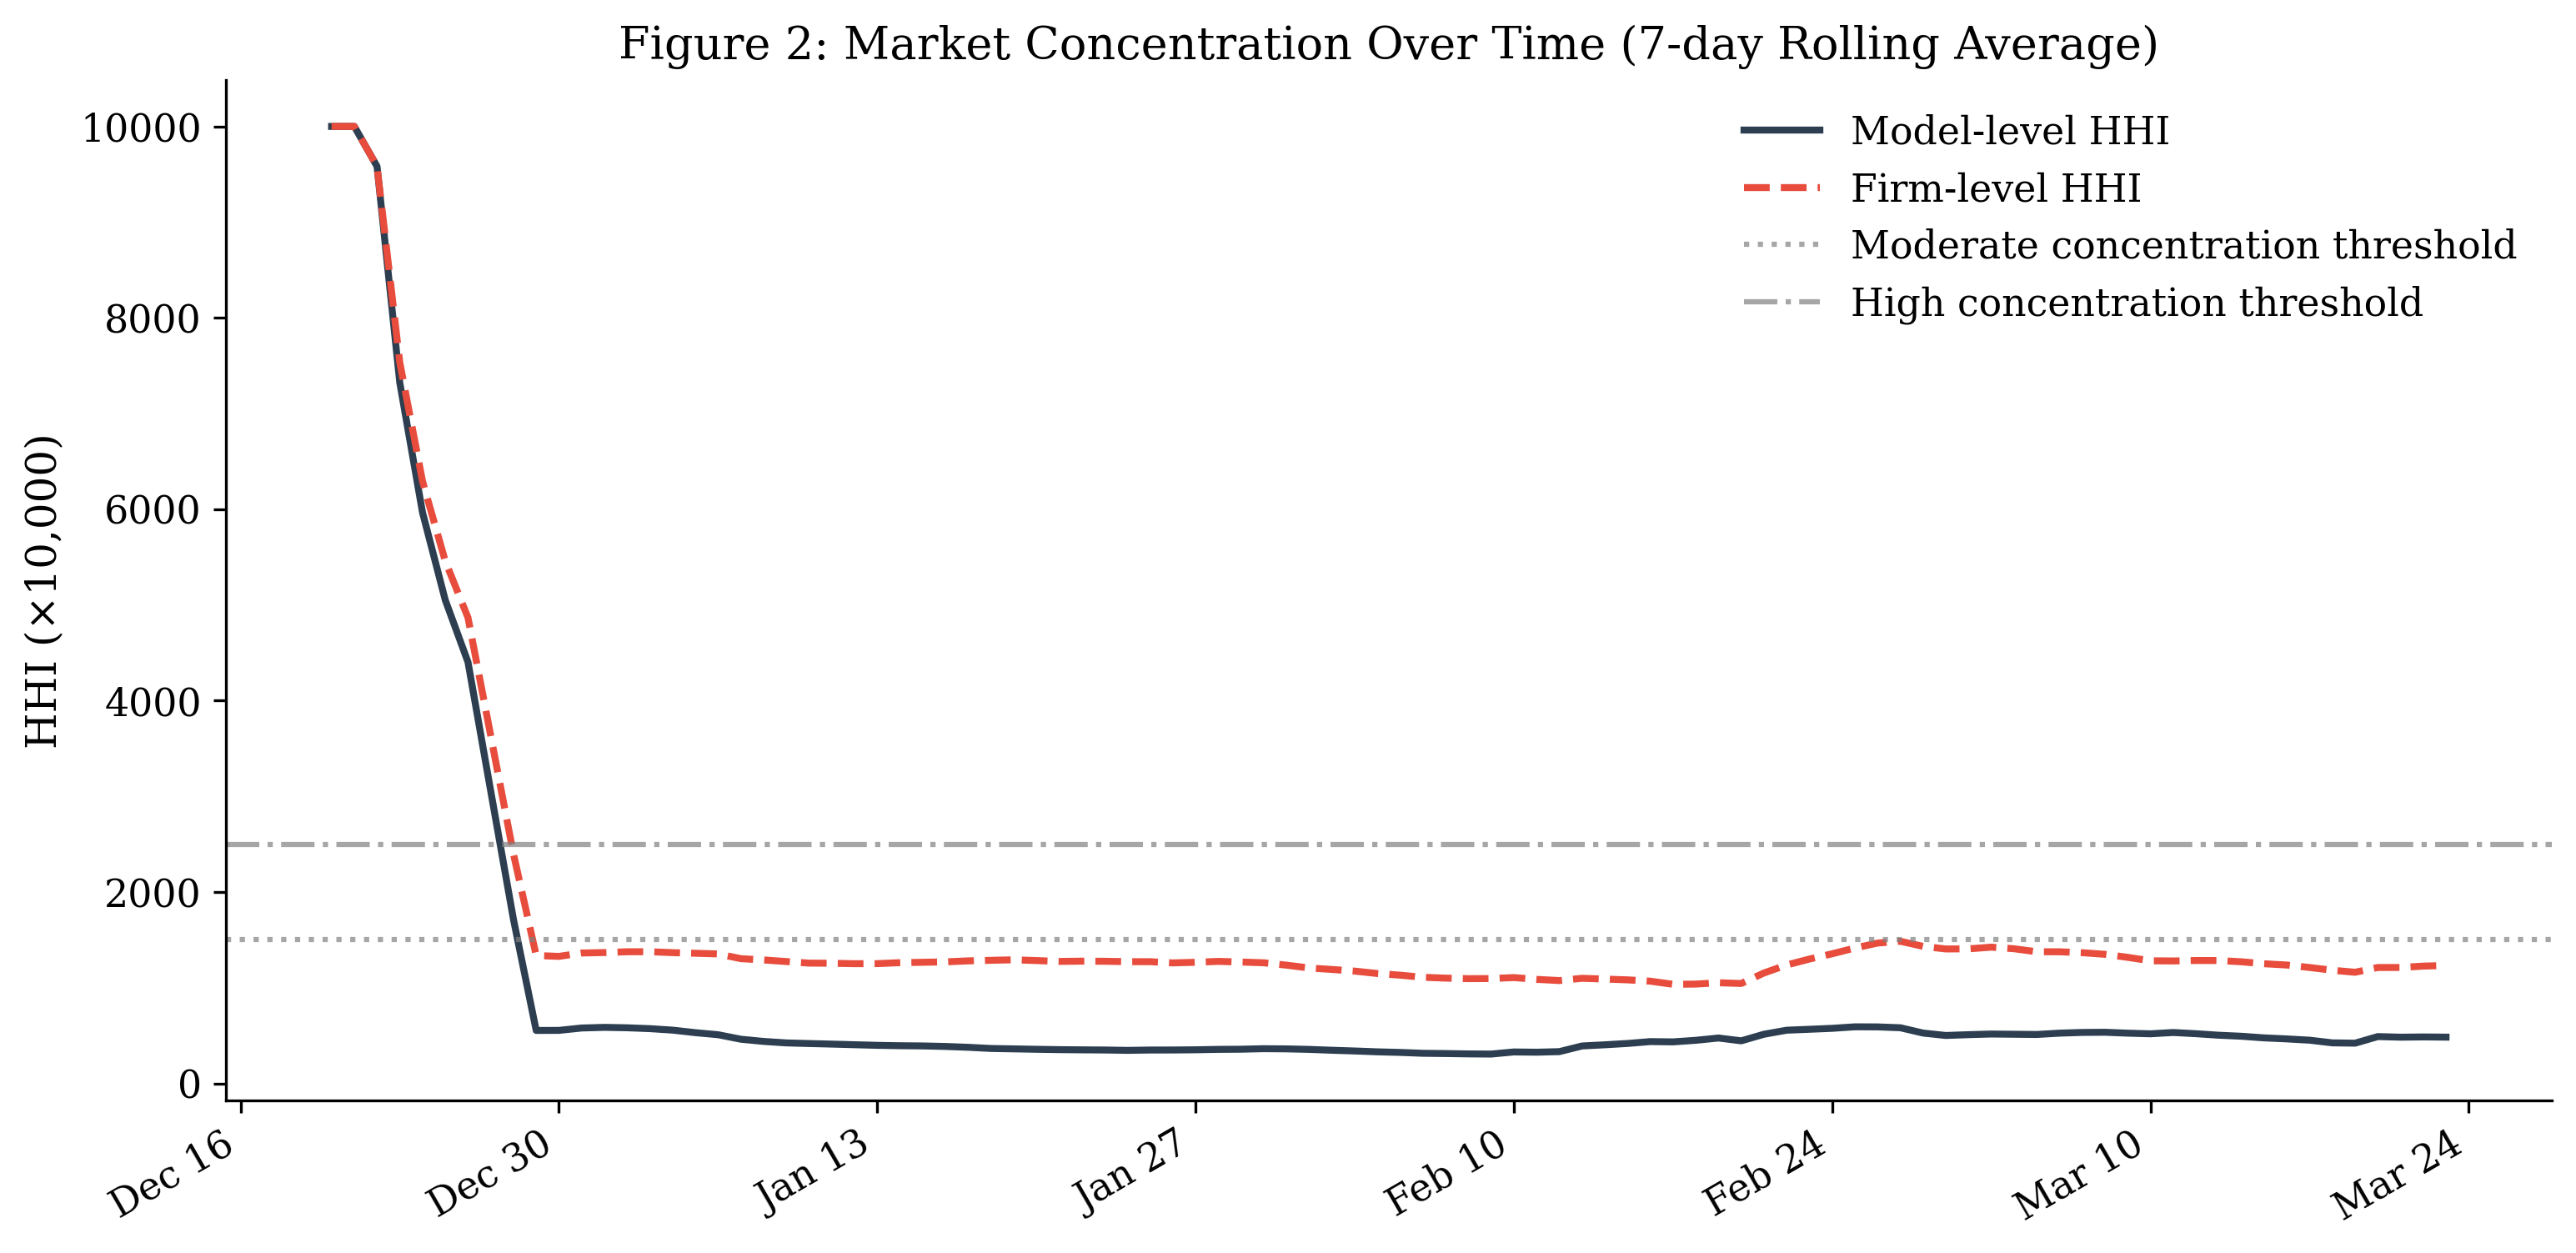
\includegraphics[width=0.85\textwidth]{../output/figures/fig02_hhi_over_time.png}
\caption{Market Concentration Over Time (HHI)}
\label{fig:hhi}
\par\noindent\small \textit{Notes}: Herfindahl-Hirschman Index computed at the model level and firm level, using daily request shares. The model-level HHI averages 741 and the firm-level HHI averages 1,524.
\end{figure}

\begin{figure}[H]
\centering
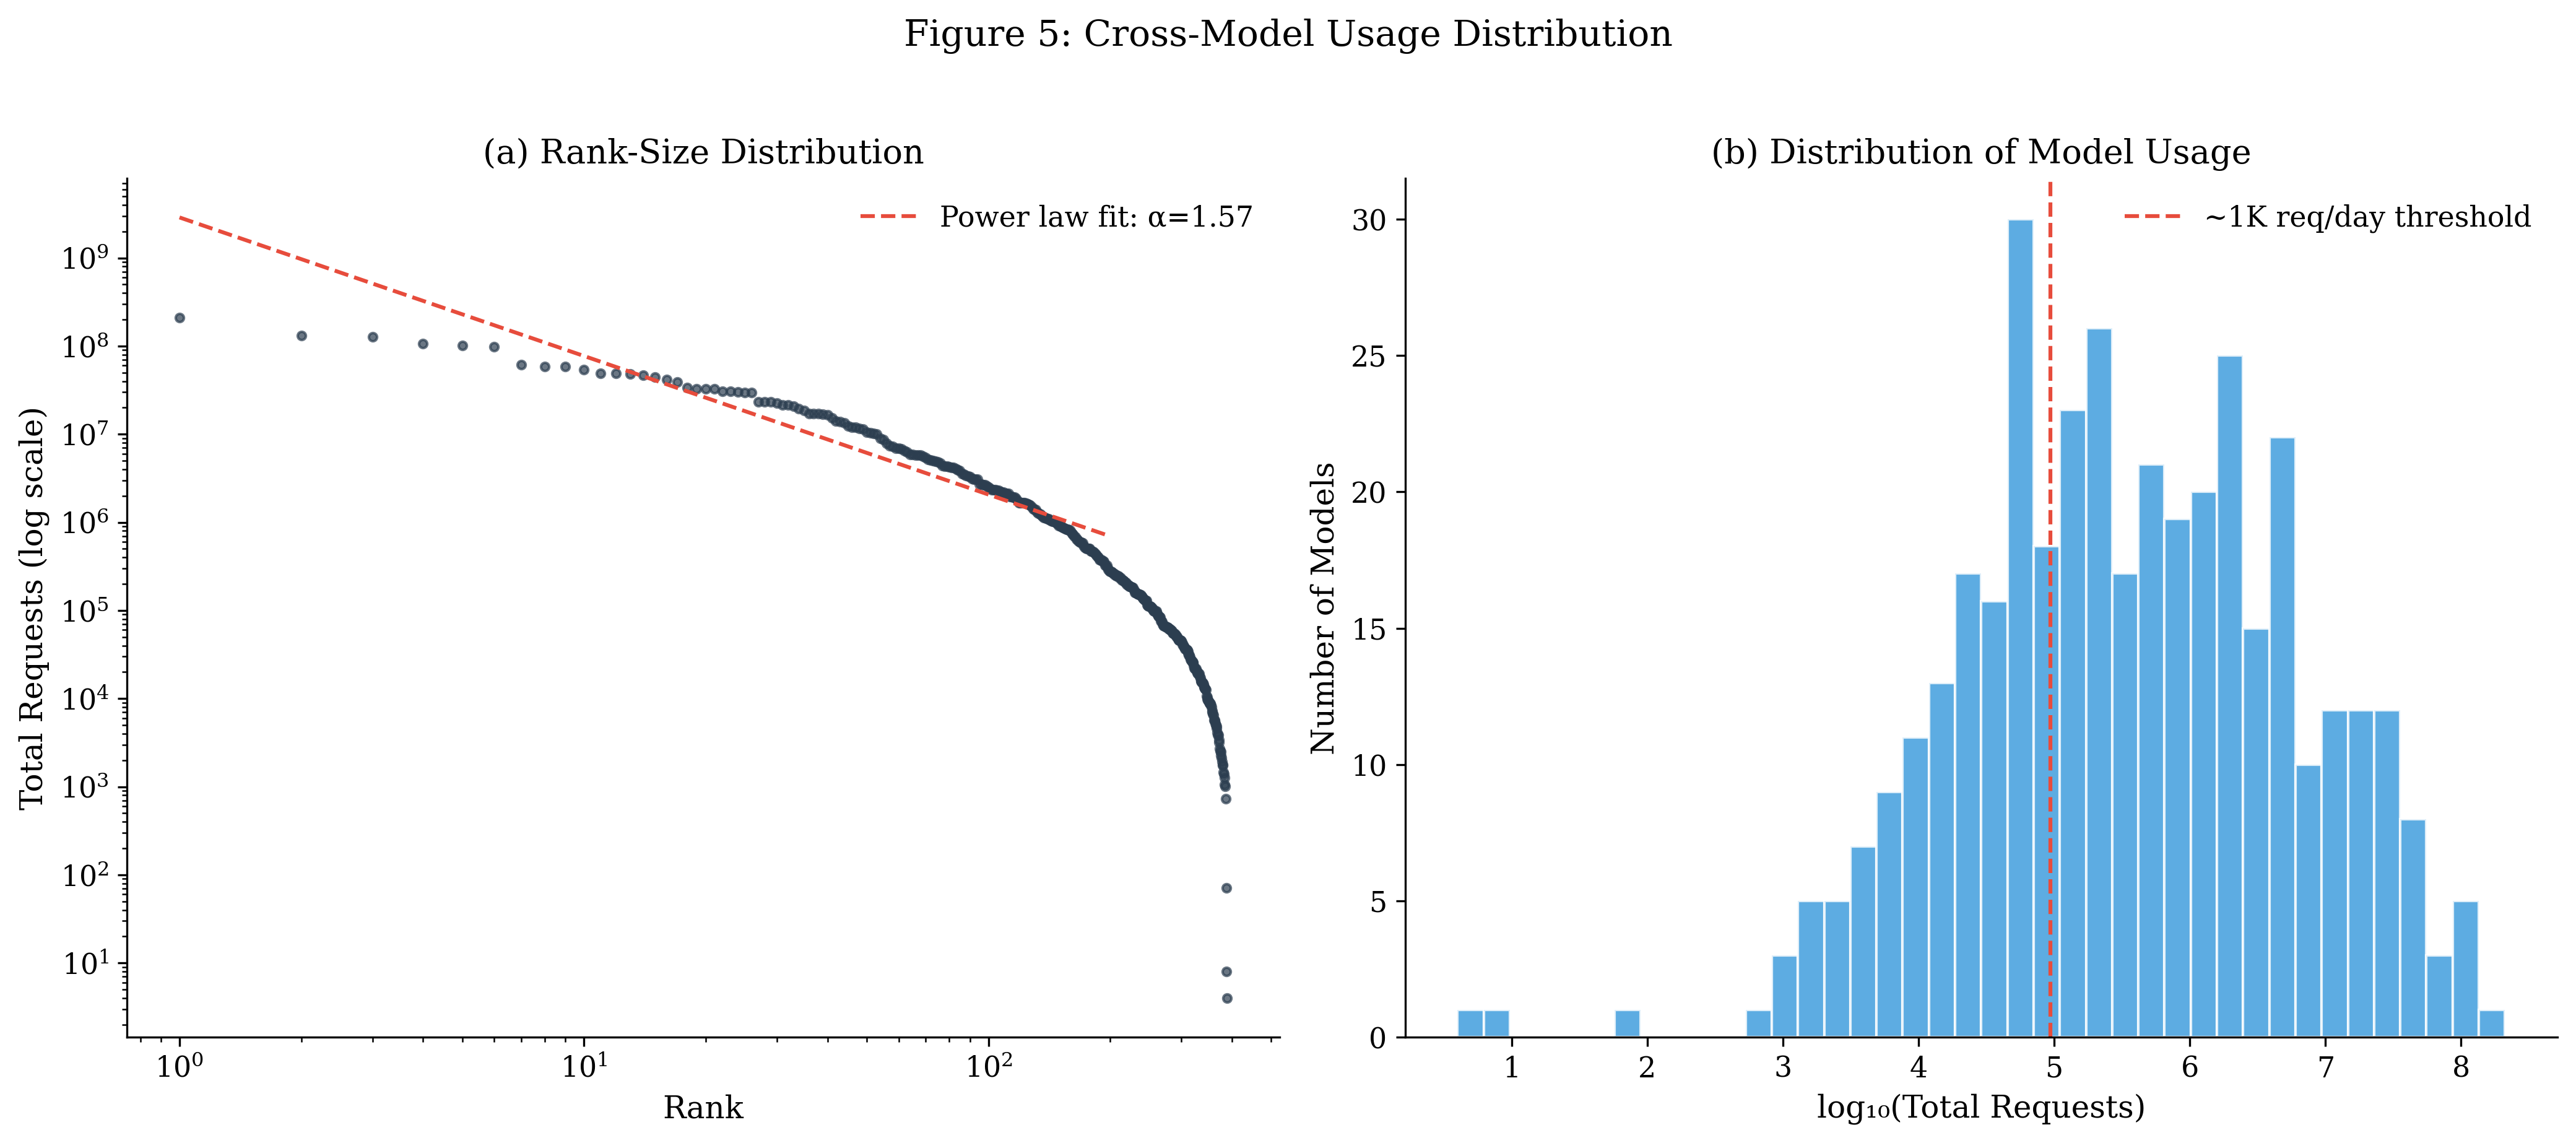
\includegraphics[width=0.85\textwidth]{../output/figures/fig05_usage_distribution.png}
\caption{Rank-Size Distribution of Model Usage}
\label{fig:ranksize}
\par\noindent\small \textit{Notes}: Log-log plot of model rank (by total requests) against total requests over the sample period. The fitted power-law exponent is $\alpha = 1.57$.
\end{figure}

\begin{figure}[H]
\centering
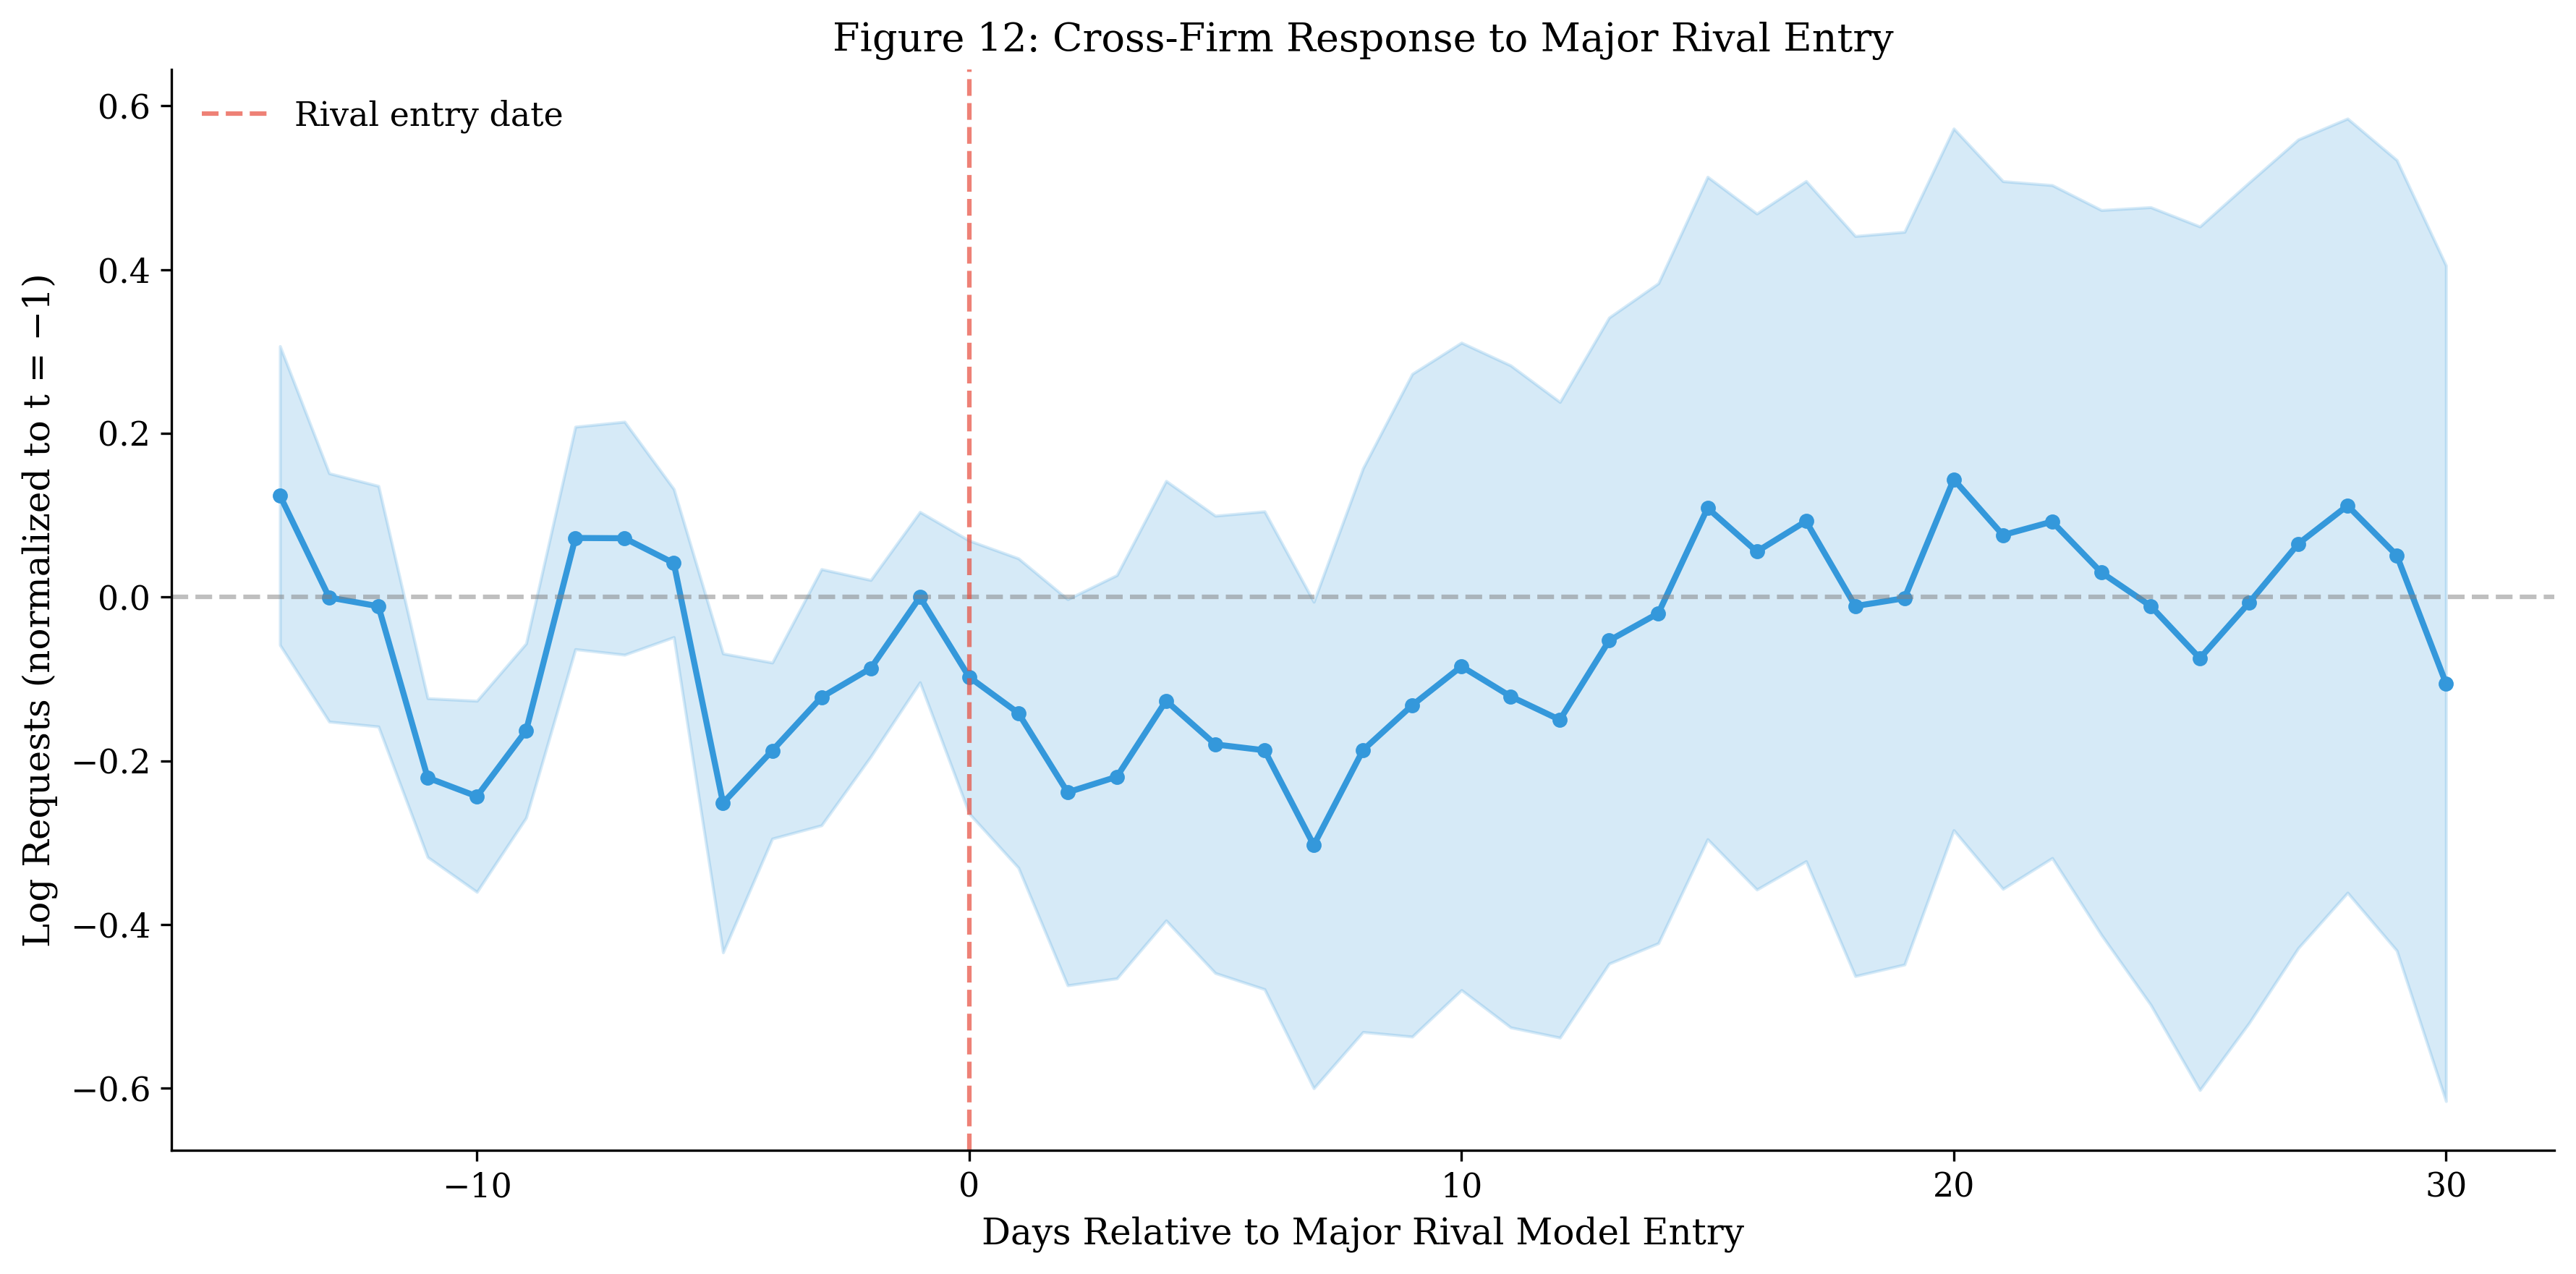
\includegraphics[width=0.85\textwidth]{../output/figures/fig12_event_study_cross_firm.png}
\caption{Event Study: Cross-Firm Entry}
\label{fig:es_cross}
\par\noindent\small \textit{Notes}: Event study coefficients for incumbent model usage around cross-firm entry events. Reference period is $k = -1$. Post-entry coefficients are negative on average but noisy and not significantly different from zero.
\end{figure}

\begin{figure}[H]
\centering
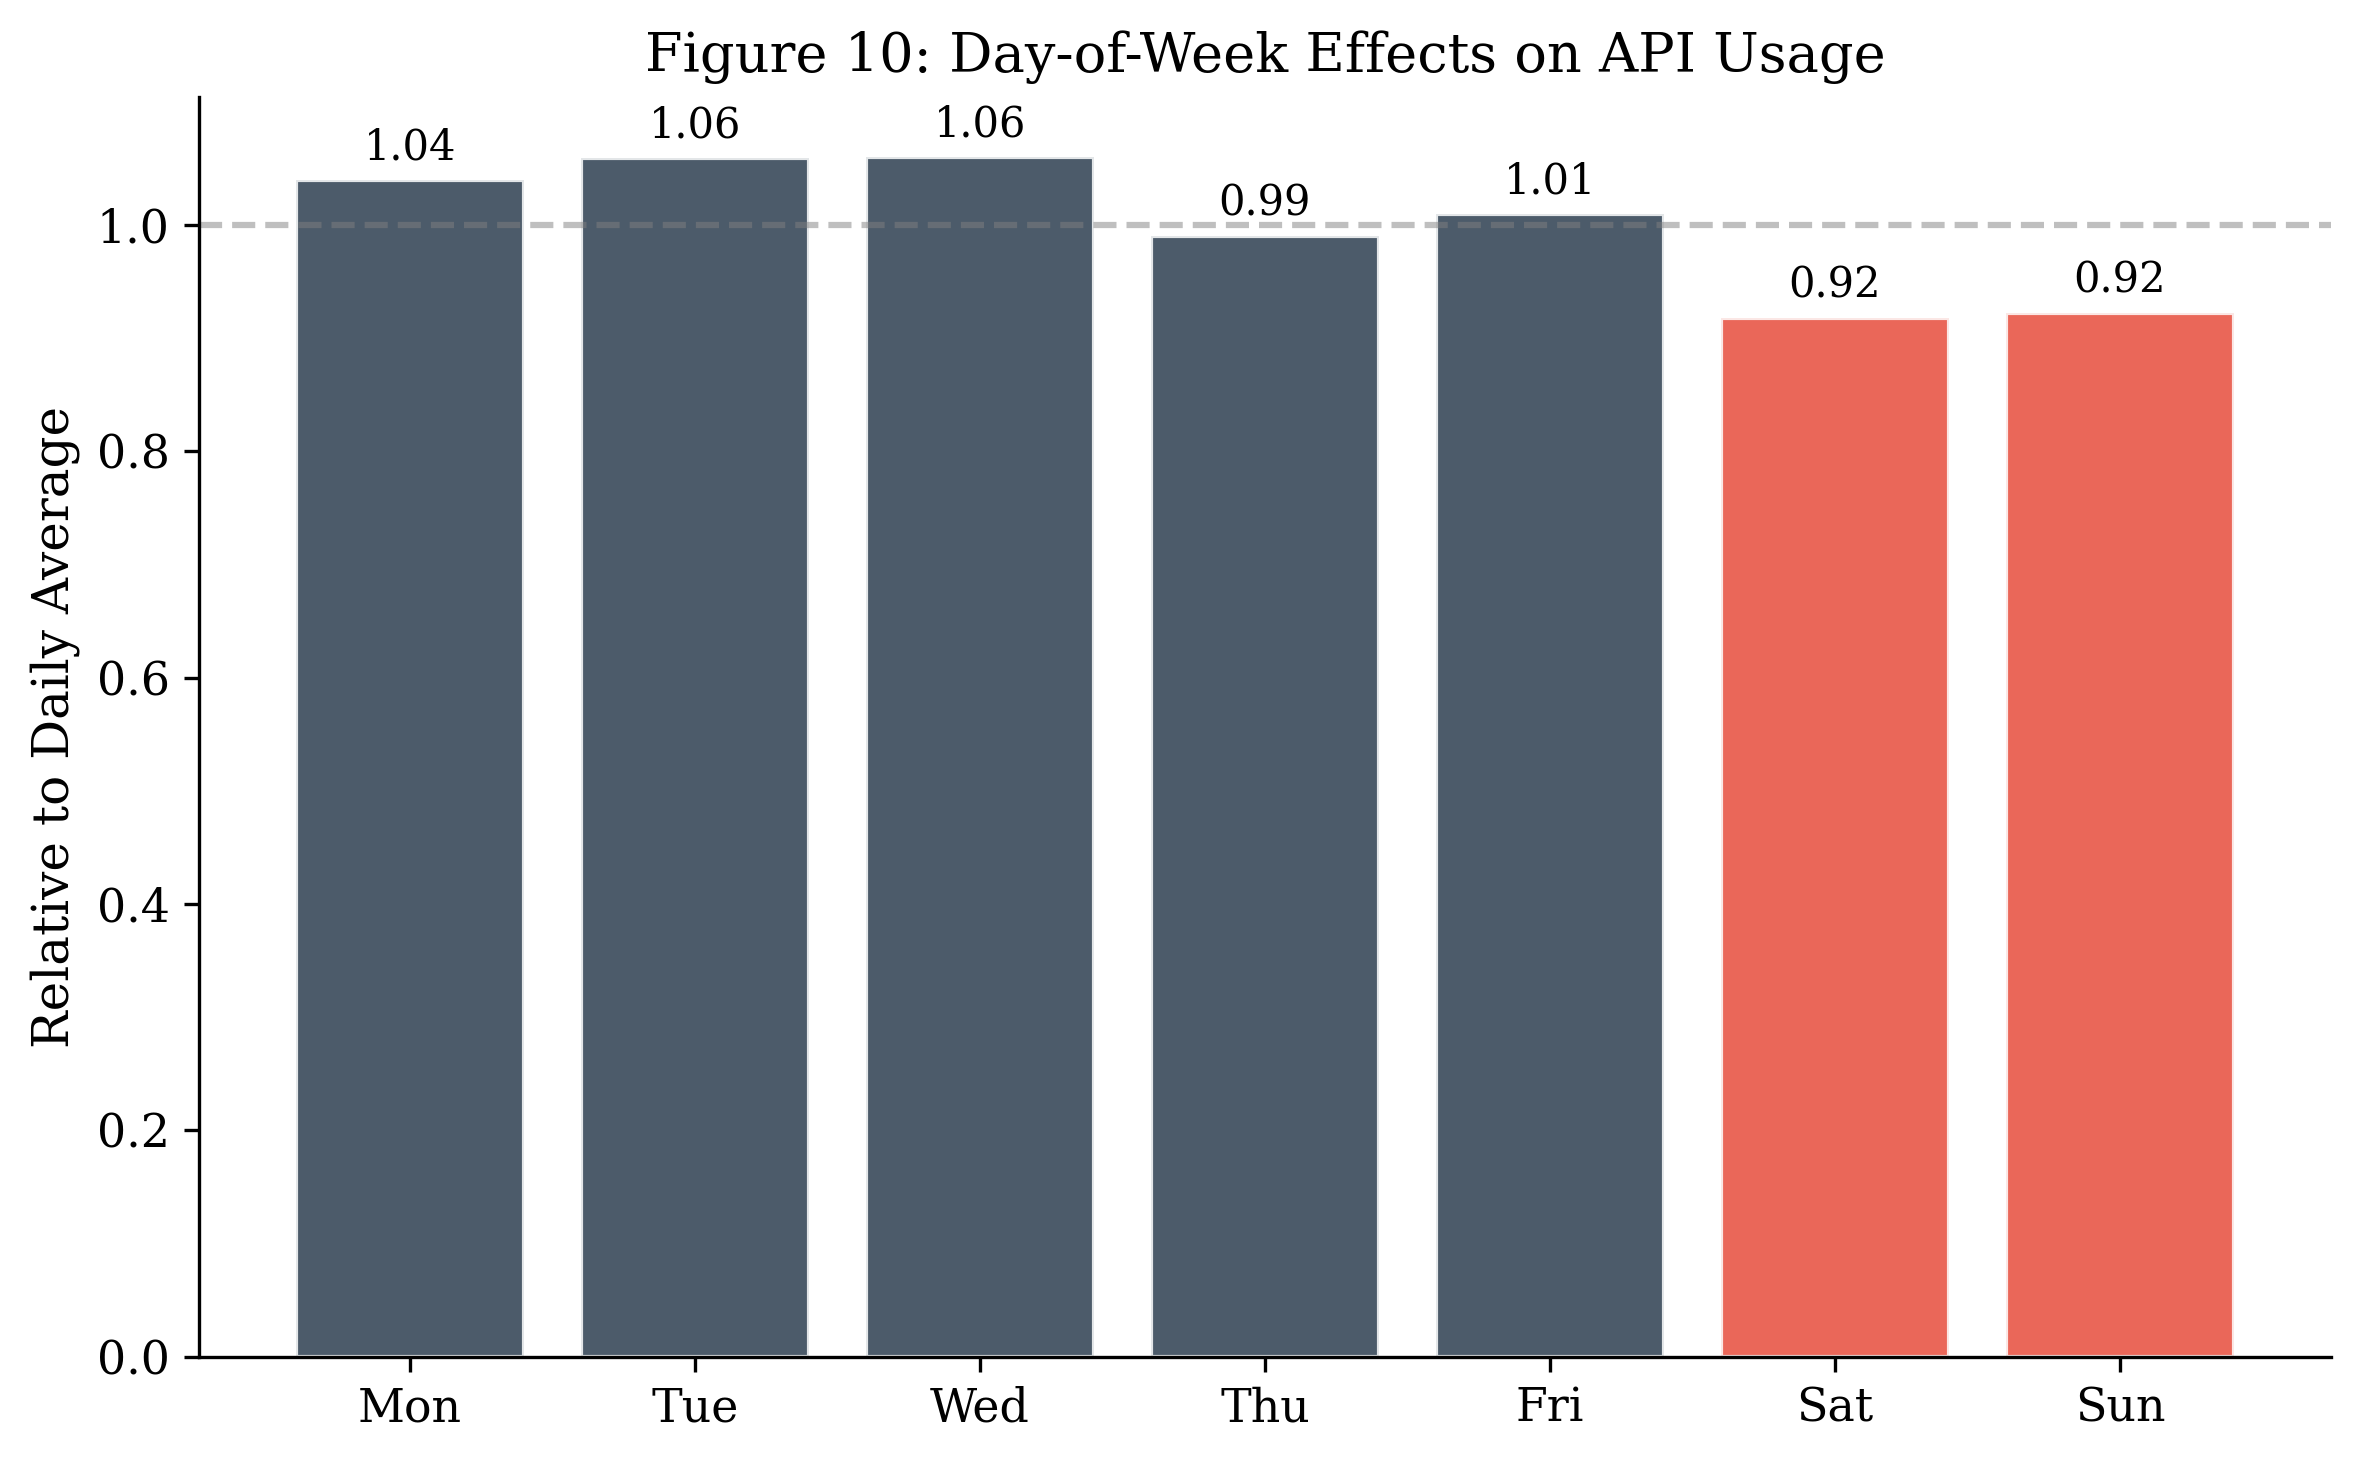
\includegraphics[width=0.85\textwidth]{../output/figures/fig10_weekday_effects.png}
\caption{Day-of-Week Usage Patterns}
\label{fig:weekday}
\par\noindent\small \textit{Notes}: Average daily requests by day of week, normalized to the overall daily mean. Weekdays run 3\% above average; weekends run 8\% below.
\end{figure}

\begin{figure}[H]
\centering
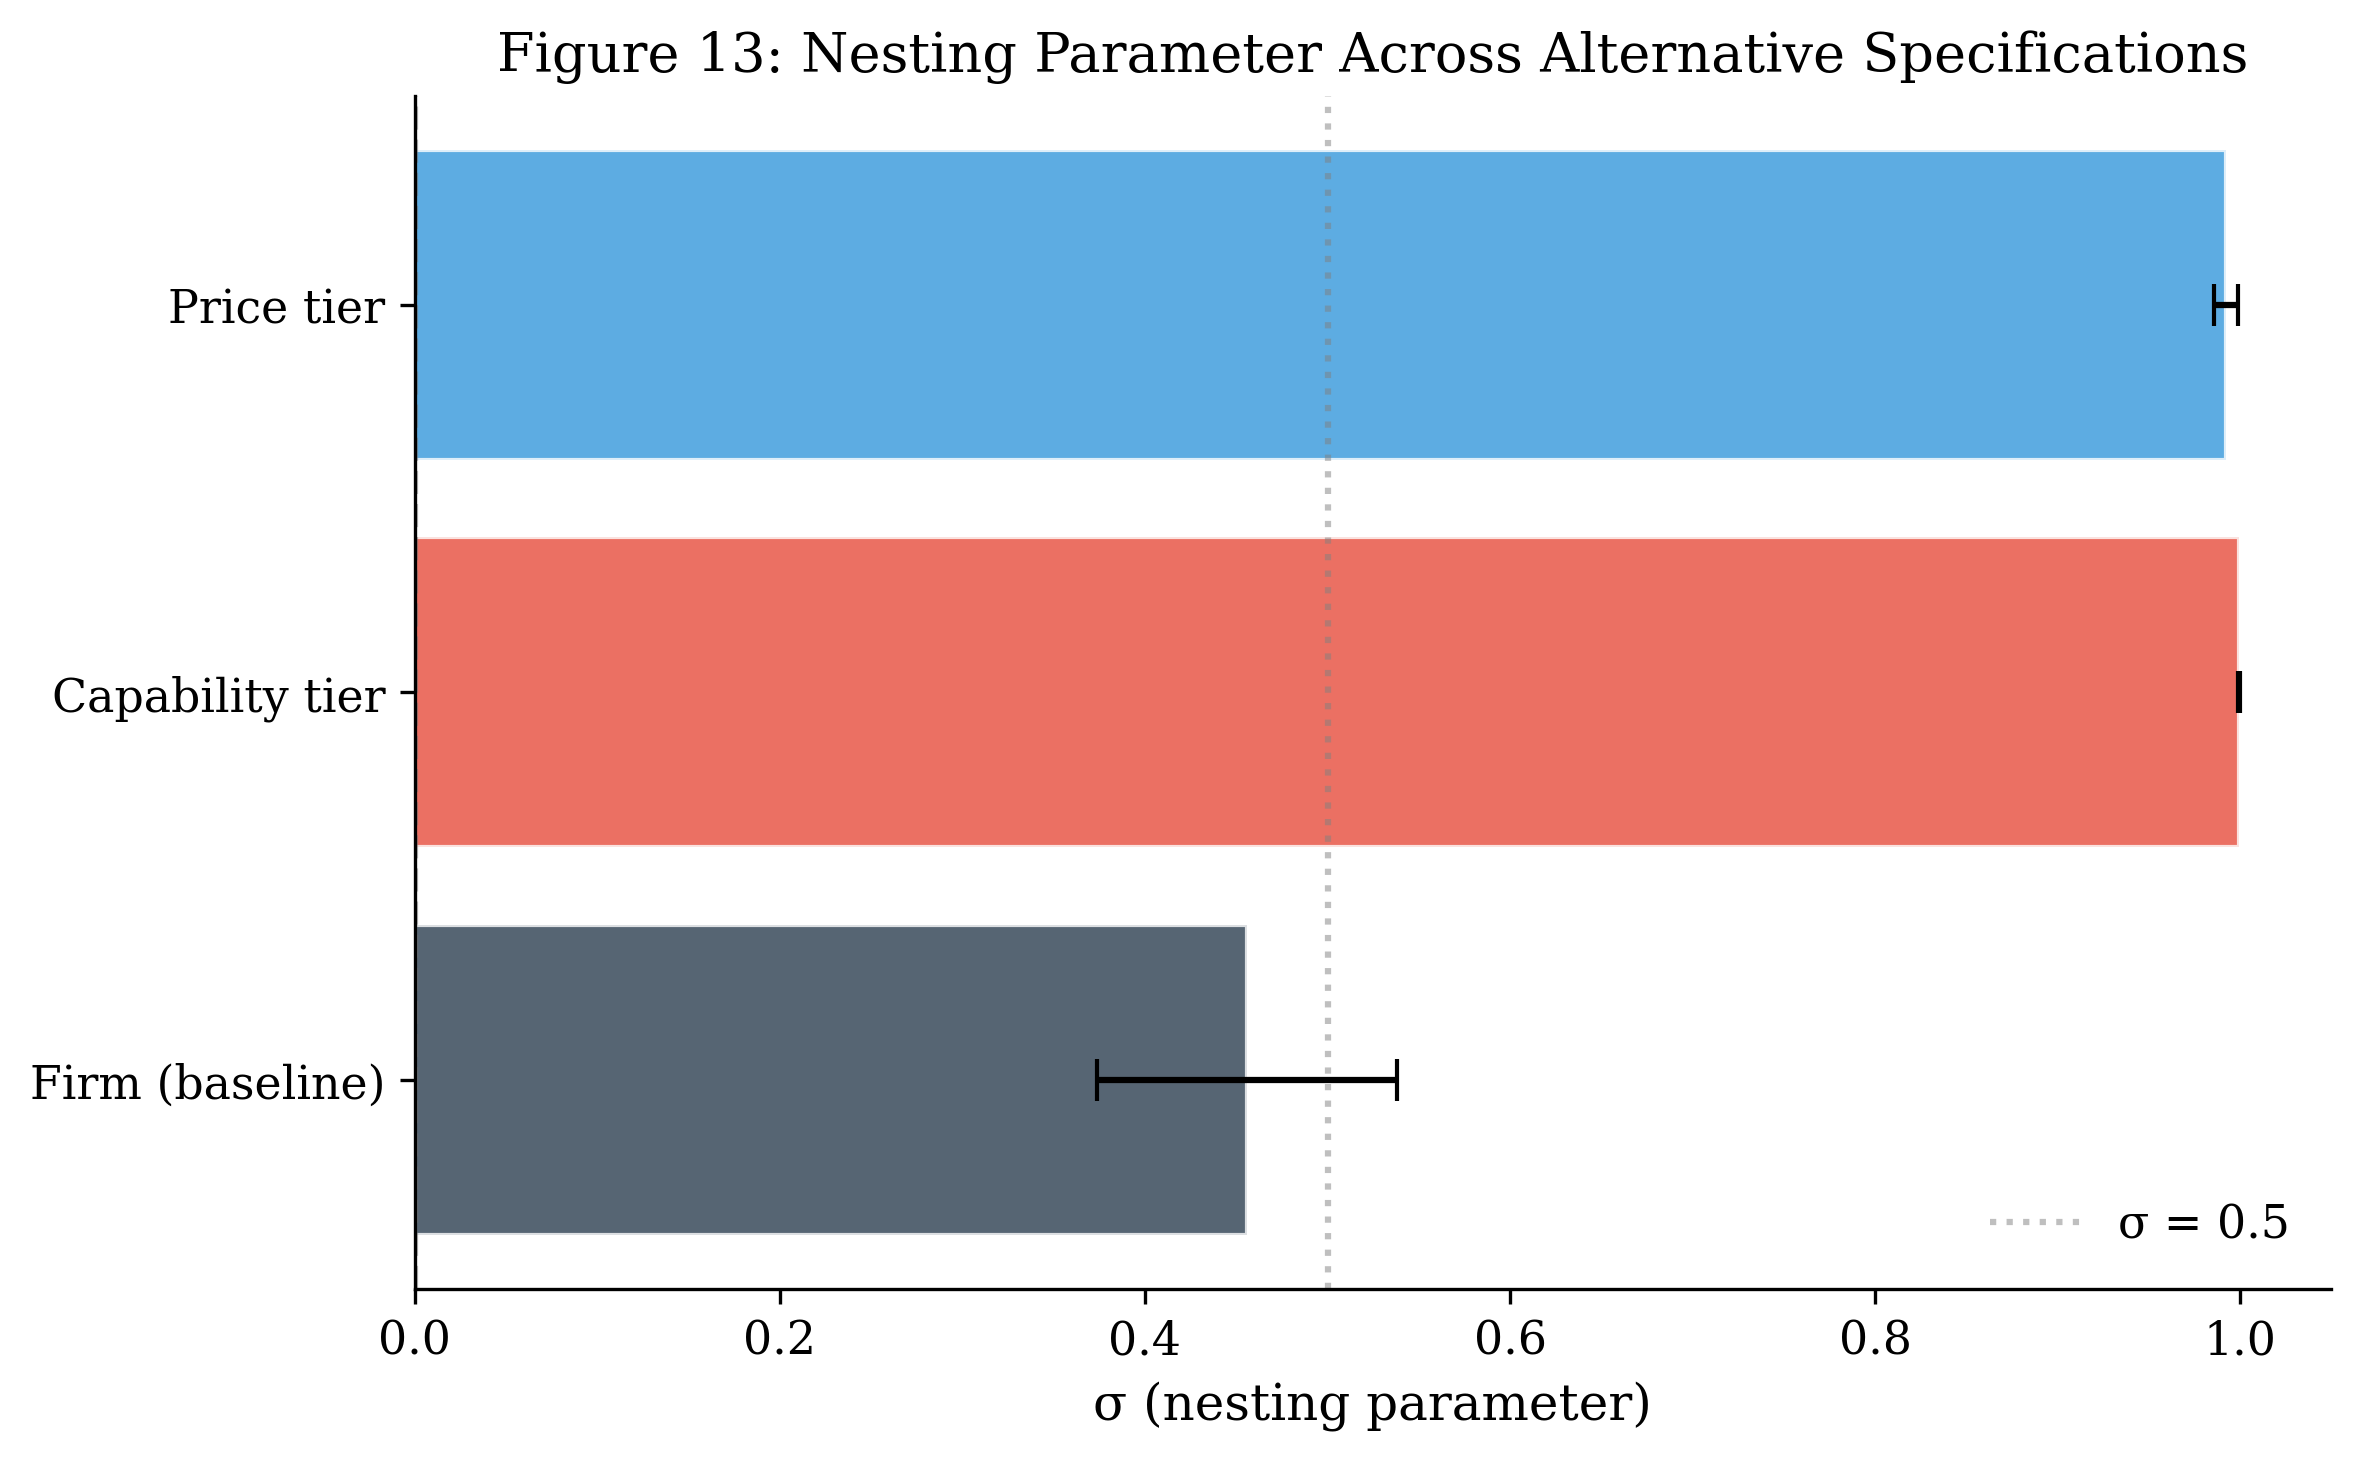
\includegraphics[width=0.85\textwidth]{../output/figures/fig13_robustness_sigma.png}
\caption{Sensitivity of Nesting Parameter to Specification}
\label{fig:sigma_robust}
\par\noindent\small \textit{Notes}: Estimated nesting parameter $\hat{\sigma}$ under alternative specifications: baseline firm-based nesting, reasoning-only subsample, non-reasoning subsample, capability-tier nesting, and price-tier nesting. Error bars show 95\% confidence intervals.
\end{figure}

\begin{figure}[H]
\centering
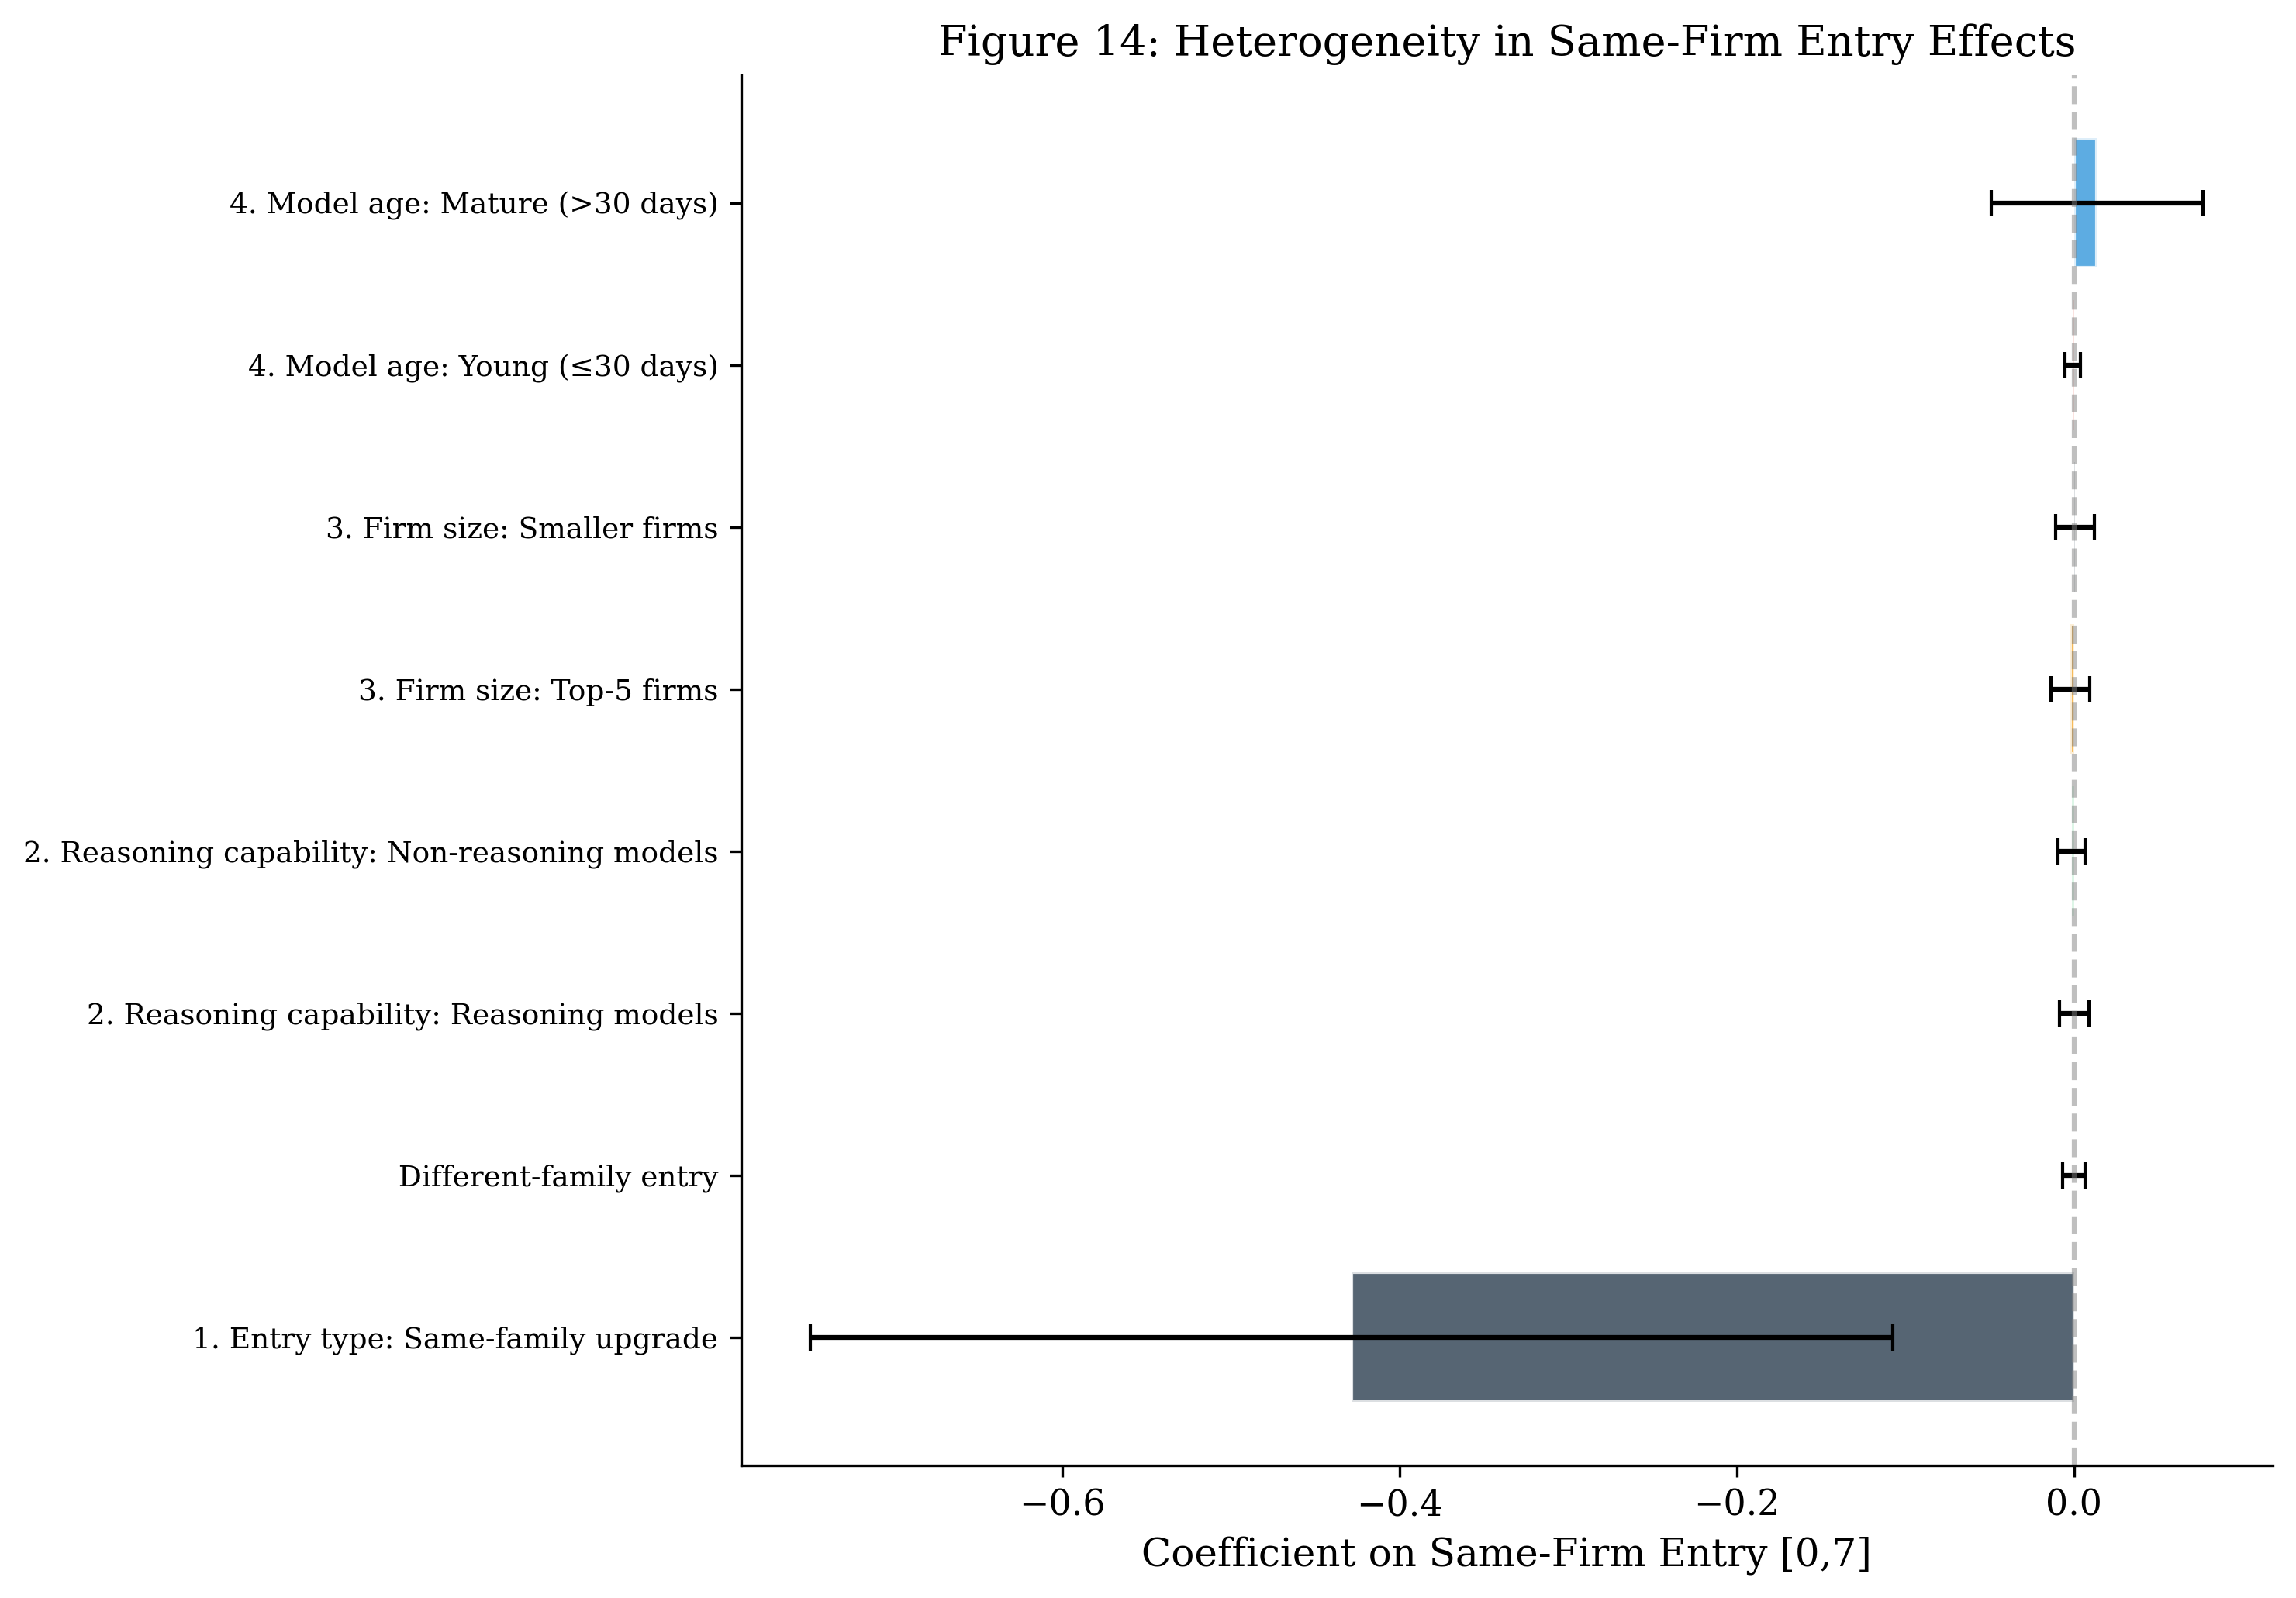
\includegraphics[width=0.85\textwidth]{../output/figures/fig14_heterogeneity.png}
\caption{Heterogeneity in Same-Firm Entry Effects}
\label{fig:het}
\par\noindent\small \textit{Notes}: Same-firm entry $[0,7]$ coefficient estimated separately by subgroup. Error bars show 95\% confidence intervals. The same-family upgrade effect ($-0.43$) is the only statistically significant displacement channel.
\end{figure}

\section{Additional Tables}

\begin{table}[H]
\centering
\caption{Leave-One-Firm-Out Sensitivity}
\label{tab:lofo}
\begin{threeparttable}
\begin{tabular}{lrrr}
\toprule
Excluded firm & $\hat{\beta}$ & SE & $N$ \\
\midrule
Google & $-0.000$ & (0.003) & 28,813 \\
OpenAI & $-0.005$ & (0.005) & 25,514 \\
Mistral & $0.001$ & (0.003) & 28,010 \\
Minimax & $-0.000$ & (0.003) & 30,399 \\
DeepSeek & $-0.001$ & (0.003) & 29,834 \\
\bottomrule
\end{tabular}
\begin{tablenotes}[flushleft]
\small
\item \textit{Notes}: Same-firm entry $[0,7]$ coefficient from equation~\eqref{eq:panel}, re-estimated after excluding all models from the named firm. Model and day fixed effects included. Standard errors clustered at the model level.
\end{tablenotes}
\end{threeparttable}
\end{table}

\section{Data Cleaning and Sample Construction Details}

The raw daily usage panel contains 29,407 rows. We apply the following cleaning steps:
\begin{enumerate}[nosep]
\item Remove duplicate model--date entries (323 rows removed).
\item Exclude the most recent calendar day's data, which may be incomplete due to the platform's retroactive update process.
\item Merge model metadata (firm identity, characteristics, pricing) using model identifiers.
\item Compute derived variables: market shares, within-firm shares, entry indicators, model age.
\item For the nested logit sample, restrict to observations where the outside option share is positive and the within-firm share is well-defined (model appears on a day when at least one other same-firm model also appears). This yields $N = 26{,}444$.
\item For the panel regression sample, retain all models with at least 1,000 total requests. This yields $N = 30{,}903$.
\end{enumerate}

All data cleaning decisions were specified in the pre-analysis plan before estimation. One deviation from the plan: the \texttt{model\_age} variable was dropped from panel specifications with model and day fixed effects, as it is perfectly collinear with the interaction of model identity and calendar date. We retain it in the nested logit specification, which does not include model fixed effects.

\section{Pre-Analysis Plan Deviations}

We document three deviations from the pre-analysis plan:
\begin{enumerate}[nosep]
\item \textbf{Model age dropped from panel regressions.} \texttt{model\_age} is a deterministic function of model identity and date, making it collinear with model $\times$ day fixed effects. This was anticipated as a possibility in the plan.
\item \textbf{Rival entry dropped from TWFE specifications.} The rival entry variable varies only by date (all models face the same number of rival entries on a given day), making it collinear with day fixed effects. We instead estimate the rival entry effect using an entity $\times$ week fixed effects specification that allows sufficient variation.
\item \textbf{Same-family vs.\ different-family decomposition added.} This was not pre-specified but is motivated by the economic distinction between vertical upgrades and horizontal diversification. It is our key finding and is robust across specifications.
\end{enumerate}

\end{appendices}

\end{document}
